% !TeX spellcheck = <none>

%contains all the imports and configurations 

\documentclass[10pt,a4paper]{report}
\usepackage[a4paper, left=2cm, right=2cm, top=2cm, bottom=2cm]{geometry}
\usepackage[utf8]{inputenc}		%utf8 allows also for umlauts
\usepackage[arabic, english]{babel}
\usepackage{amsmath}

%Declare new math operators with amsmath:

%atan2 function
\DeclareMathOperator{\atantwo}{atan2}
\DeclareMathOperator{\arctantwo}{arctan2}
\DeclareMathOperator{\acos}{acos}


\usepackage{amsfonts}
\usepackage{amssymb}
\usepackage{graphicx}	%for importing images
\graphicspath{ {./images/} {../GeneratedPlots/} }
\usepackage{gensymb}
\usepackage{siunitx}
%\usepackage{matlab-prettifier}
\usepackage{float}
\usepackage[usenames,dvipsnames]{color} % color text

%coloured text
\usepackage{xcolor} %\textcolor{blue}{This is a sample text in blue.}

\usepackage{listings}
\usepackage{alphalph}

\usepackage{breqn} %automatic linebreaking math environment
%insert after all math stuff e.g. amsmath, amssymb mathpazo... is imported

%insert external pdf pages in document
\usepackage{pdfpages} 
% http://texdoc.net/texmf-dist/doc/latex/pdfpages/pdfpages.pdf

%Bibliography settings
\usepackage[citestyle = numeric, style=numeric, bibstyle = numeric]{biblatex} 
\addbibresource{References.bib}    

% for including current date into document
\usepackage[ddmmyyyy]{datetime}

%Give captions to items that normally don't have any
\usepackage{caption} 
%use as:
%\DeclareCaptionType{exam}[Example][List of Examples]
%\listofexams
%\begin{enumerate}
%	\item First item.
%	\item Second item.
%	\item Third item.
%	\captionof{exam}{This is a very important list.}
%\end{enumerate}

%For making an appendix
\usepackage[toc,page]{appendix}

% \usepackage[table,xcdraw]{xcolor}

%line drawing in array or tabular
%\usepackage{arydshln} %here used for mimicing matrices in array with dashed lines
%Doesn't work as intended

%Matrix options for dotted lines, etc. etc...
\usepackage{nicematrix} % here used for makin g arrays with dashed separator lines
%http://ctan.math.washington.edu/tex-archive/macros/latex/contrib/nicematrix/nicematrix.pdf

\usepackage{enumitem}
\usepackage{multicol}%try it out!





%acronym package (needs an acronym chapter)
\usepackage{acronym}
%\usepackage{acro}	%Alternative, more elaborate package for acronyms
%\acsetup{hyperref = true, only-used = true, sort = true,  }

\DeclareAcronym{HAN}{short = HAN , long = Hogeschool van Arnhem en Nijmegen }
\DeclareAcronym{SPC}{short = SPC , long = Smart Production Cell }
\DeclareAcronym{PC}{short = PC , long = Personal Computer }
\DeclareAcronym{DOF}{short DOF = , long = Degree of Freedom }






%\begin{acronym}[Bash]

%	\acro{HAN}{Hogeschool van Arnhem en Nijmegen}
%	\acro{SPC}{Smart Production Cell}
%	\acro{DOF}{degrees of freedom}
%	\acro{FRC}{Fibre Reinforced Composites}
%	\acro{DH}{Denavit-Hartenberg}
%	\acro{IOT}{Internet Of Things}
%	\acro{FHEM}{Freundliche Hausautomation und Energie-Messung \cite{FHEM}}
%	\acro{NFC}{Near-field communication}
%	\acro{IPKW}{Industrial Park Kleevse Waard}
%	\acro{NFC}{Near Field Communication}
%	\acro{ROS}{Robot Operating System}
%	\acro{GUI}{Graphical User Interface}
%	\acro{EOAT}{End Of Arm Tooling}
%	\acro{PL}{Production Line}
%	\acro{ETCS}{European Train Control System}
%	\acro{DT}{Digital Twin}
%	\acro{eq}{equation}
%	\acro{DCS}{Dual Check Safety}
%	\acro{DDS}{Data Distribution System}
%	\acro{fig}{figure}
%	\acro{sect}{section}
%	\acro{OS}{Operating System}
%\end{acronym}


%import PDF pages
\usepackage{pdfpages}
%To include all the pages in the PDF file:
%\includepdf[pages=-]{myfile.pdf}
%To include just the first page of a PDF:
%\includepdf[pages={1}]{myfile.pdf}

%Start new chapter on same page to avaoid big spaces
\usepackage{etoolbox}
\makeatletter
\patchcmd{\chapter}{\if@openright\cleardoublepage\else\clearpage\fi}{}{}{}
\makeatother


\newcommand*\wildcard[2][6cm]{\vspace*{2cm}\parbox{#1}{\hrulefill\par#2}} %Wildcard for Signature line

\usepackage{lipsum} %random text

%If custom headers are needed
%\usepackage{fancyhdr}
%
%\pagestyle{fancy}
%\fancyhf{}
%\rhead{Overleaf}
%\lhead{Guides and tutorials}
%\rfoot{Page \thepage}

%for left, center or right aligning figures
\usepackage[export]{adjustbox}
%https://tex.stackexchange.com/questions/91566/syntax-similar-to-centering-for-right-and-left

%Remove word "chapter" but leave numbering
\makeatletter
\renewcommand{\@makechapterhead}[1]{%
	\vspace*{50 pt}%
	{\setlength{\parindent}{0pt} \raggedright \normalfont
		\bfseries\Huge\thechapter.\ #1
		\par\nobreak\vspace{40 pt}}}
\makeatother

%Add line below chapter title and minimze space when text starts
%\usepackage[]{titlesec}
%\titleformat{\chapter}[hang]{\huge\sffamily\bfseries}{}{0pt}{}[\hrule\vspace*{-23pt}] 

%no indentation for paragraphs
\setlength{\parindent}{0cm}

\usepackage{hyperref} %Load last as it can cause trouble with other packages. For Hyperlink https://de.wikibooks.org/wiki/LaTeX-W%C3%B6rterbuch:_hyperref
\hypersetup{
	colorlinks=true,
	linkcolor=blue,
	filecolor=magenta,      
	urlcolor=cyan,
}
\urlstyle{same} %The default is equivalent to \urlstyle{tt}; with \urlstyle{rm} and \urlstyle{sf} the font will be the roman or sans serif upright font. With \urlstyle{same} the current font will be used.

\usepackage{cleveref} %multi reference with \cref{x,y}
% needs to be loaded after hyperref 

%Making a Glossary
\usepackage{glossaries}
%\usepackage[xindy]{glossaries}
%\usepackage[style=long,toc,automake]{glossaries}
%https://en.wikibooks.org/wiki/LaTeX/Glossary
%http://tug.ctan.org/macros/latex/contrib/glossaries/glossariesbegin.pdf

%\makenoidxglossaries

\newglossaryentry{latex}
{
	name=latex,
	description={Is a mark up language specially suited 
		for scientific documents}
}

\newglossaryentry{maths}
{
	name=mathematics,
	description={Mathematics is what mathematicians do}
}


\makeglossaries

%Set some things clear 
\newcommand{\HANSupervisor}{Wesselingh Ellen}
\newcommand{\CompanySupervisor}{Nguyen Trung}
\author{Karl Wallkum}

%% Preamble 
%Deactivate before Distribution!!




















%\documentclass[10pt,a4paper]{report}
%\usepackage[a4paper, left=2cm, right=2cm, top=2cm, bottom=2cm]{geometry}
%\usepackage[utf8]{inputenc}		%utf8 allows also for umlauts
%\usepackage[arabic, english]{babel}
%
%\usepackage{hyperref} %Load last as it can cause trouble with other packages. For Hyperlink https://de.wikibooks.org/wiki/LaTeX-W%C3%B6rterbuch:_hyperref
%\hypersetup{
%	colorlinks=true,
%	linkcolor=blue,
%	filecolor=magenta,      
%	urlcolor=cyan,
%}
%\urlstyle{same} %The default is equivalent to \urlstyle{tt}; with \urlstyle{rm} and \urlstyle{sf} the font will be the roman or sans serif upright font. With \urlstyle{same} the current font will be used.
%
%
%\usepackage{glossaries}
%\newglossaryentry{latex}
{
	name=latex,
	description={Is a mark up language specially suited 
		for scientific documents}
}

\newglossaryentry{maths}
{
	name=mathematics,
	description={Mathematics is what mathematicians do}
}

%\makeglossaries
%
\title{How to create a glossary}
\author{ }
\date{ }


\begin{document}
	\pagenumbering{roman}
		
	\begin{titlepage}
	\begin{flushright}
	\begin{minipage}{\linewidth}
		\begin{figure}[H]
			\begin{flushright}
			
\includegraphics[width=0.5\linewidth]{Images/HAN}
			%\caption{This is the first figure}
		\end{flushright}
		\hrule
		\end{figure}
		\begin{flushright}
			\large\textbf{ HAN Master Major Project}\\
			\vspace{20pt}
			\Huge\textbf{Major Project Plan
			\\
			\vspace{10pt}
			Using FANUC R-2000iC/210F\\
			(6-axis robot) for improved efficiency in FRC parts formation }
		\end{flushright}
		\vspace{35pt}
		\begin{figure}[H]
		\begin{flushleft}
		%	\includegraphics[width=0.25\linewidth]{Images/HAN_merk}
			%\caption{This is the second figure}
		\end{flushleft}	
		\end{figure}
		\begin{itemize}[leftmargin=4.5cm]
			\LARGE	
			\item[\textbf{Student Number:}] 617931		
			\item[\textbf{Name:}] Karl Wallkum 			
			\item[\textbf{Track:}] Master Control Systems Engineering
			\item[\textbf{Company:}]  HAN Smart Production Cell (IPKW)
			\item[\textbf{Supervisors:}]  \CompanySupervisor, (Company Supervisor)\\ \HANSupervisor, (HAN Supervisor)			
			\item[\textbf{Date:}] \today		 		
		\end{itemize}
	\end{minipage}
	\end{flushright}

	\begin{flushleft}
	\large \textbf{
		\vspace{40pt}
		\\HAN Smart Production Cell (IPKW)
	}
	%\vspace{10pt}
%	\\Arnhem, \hrulefill
%	\hspace*{0mm}\phantom{Arnhem, }Nguyen Trung

	\end{flushleft}
%\makebox[.5\linewidth][l]{Arnhem, }\dotsign\smallskip\\
%\hspace*{.5\linewidth}Nguyen Trung\\
%\hspace*{.5\linewidth}Title...

%\tabcolsep0pt
%\hfill\begin{tabular}{r{0.5\linewidth}@{}m{0.5\linewidth}@{}}
%	Approved:~ & Approved:~ \\\cmidrule{2-2} \cmidrule{4-4} 
%%	& Fats Domino, Ph.D.\\
%%	& Chair of the Department of Nutrition\\
%\end{tabular}

\begingroup
\centering
\wildcard{\CompanySupervisor}
\hspace{4cm}
\wildcard{\HANSupervisor}
\par
\endgroup


%\footnotetext[0]{template minor project report}
\end{titlepage}
	\begin{figure}[H]
	\centering
	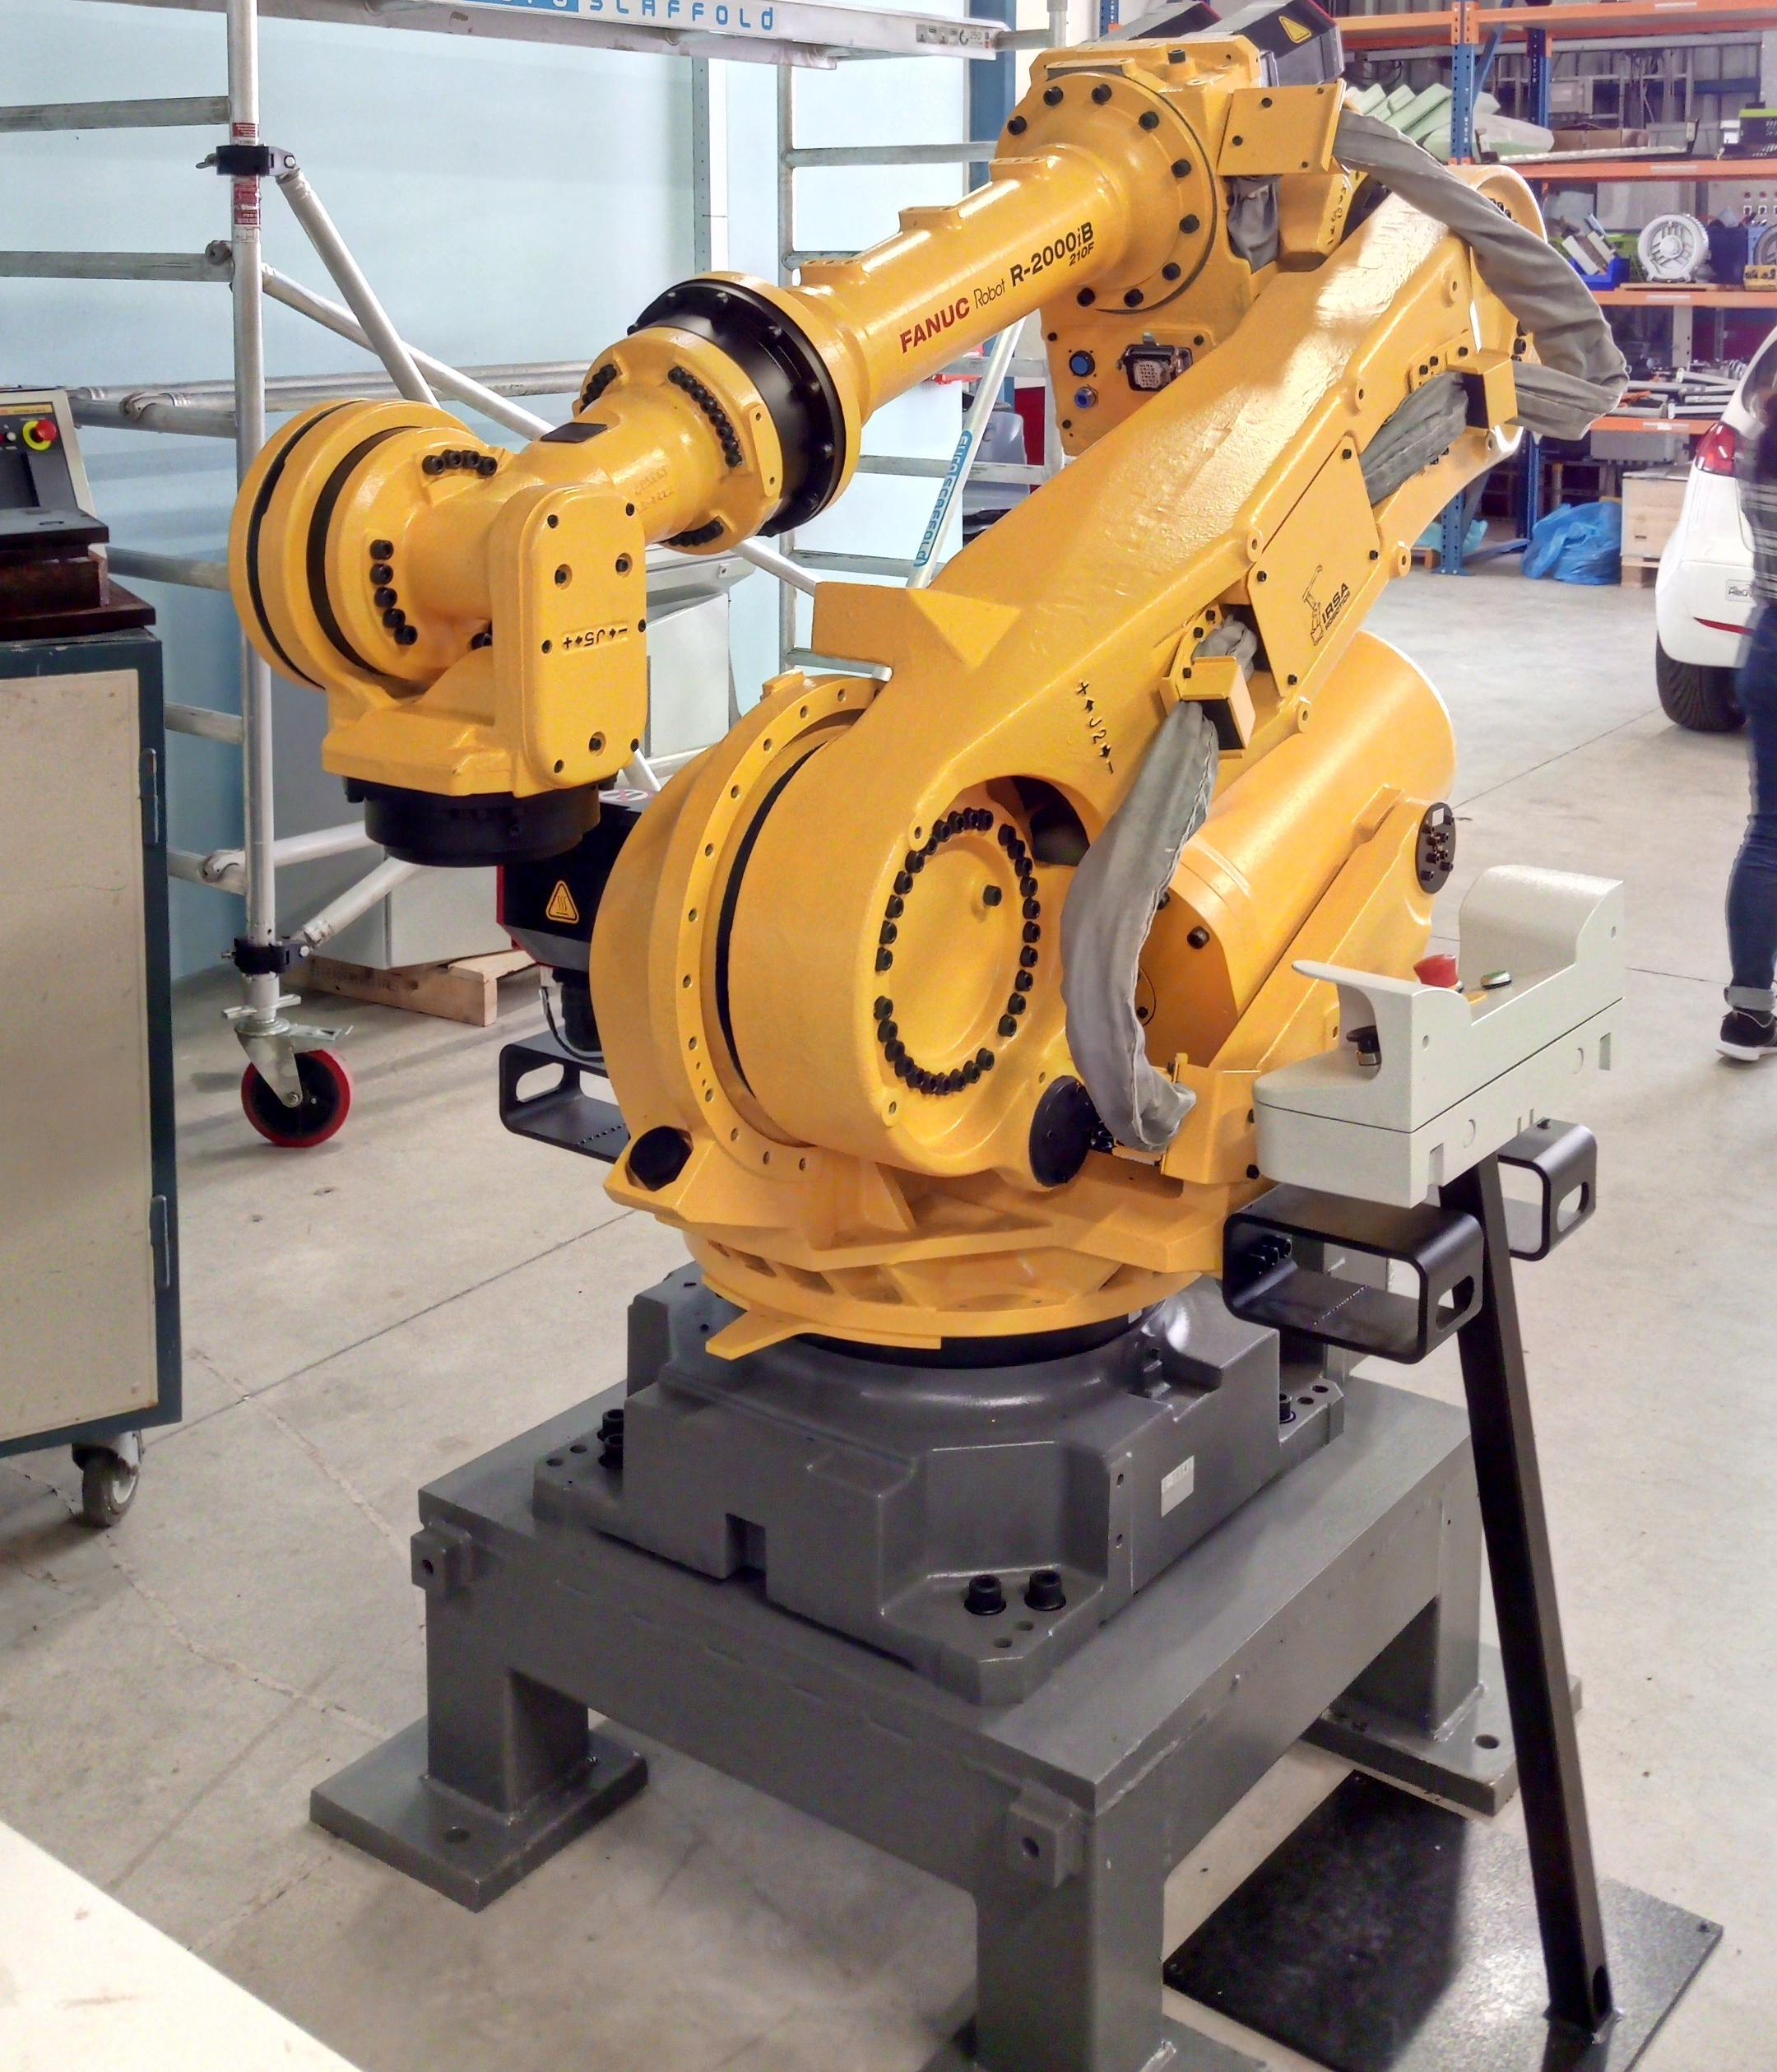
\includegraphics[
	width=1\linewidth,
	height=\paperheight,
	keepaspectratio,
	]{fanuc210_corner_cut}
	\caption{FANUC R-2000iC/210F 6-axis industrial robot arm}
	\label{fig:fanuc210}
\end{figure}
\pagestyle{empty}

	\cleardoublepage
	
	% !TeX spellcheck = <none>
%testtest
%\chapter{Summary}


	
	\newpage
	\tableofcontents
	
	\thispagestyle{empty}
	\clearpage
	\pagenumbering{arabic}
	
	%\section*{title}
The goal of this assignment is to ..\\
textextextext\\

\begin{table}[h]
	\centering
	\begin{tabular}{|l c l|}
		\hline
			&	&	\\
			&	&	\\
			&	&	\\
			&	&	\\
		\hline
	\end{tabular}
	\caption{caption}
	\label{Tab:table1}
\end{table}
%
textext as seen in Table \ref{Tab:table1} textextext.\\

\begin{figure}[H]
	\centering
	
\includegraphics[
	width=0.8\linewidth,
	height=\paperheight,
	keepaspectratio,
	]{testimage}
	\caption{Y vs X}
	\label{fig:image1}
\end{figure}

\newpage
	
	\chapter{Abstract}
%~150Words

This work aims to integrate a FANUC 210F 6 axis industrial robot arm  into an experimental production line. 
As this production line is set in a research environment, gaining a deeper understanding of all involved systems is desired.\\
\\
The dynamic behaviour of a physical system is best expressed with an analytical model.
In order to control a robot arm, a kinematic model needs to be created. With this model, a control algorithm can be derived.\\
\\
The objective of this thesis is to derive the complete inverse kinematic model of a 6 \ac{DOF} robotic arm analytically. For an exact numerical simulation of the device most steps are laid out theoretically and difficulties in the practical implementation are described.
Additionally for follow up projects this work also contains a quick start guide and a safety manual for the robot in this setting .
Finally to contribute to current research, twinning specifications will be defined.


%See: https://www.sfu.ca/~jcnesbit/HowToWriteAbstract.htm
%
%%What is an Abstract?
%
%The abstract is an important component of your thesis. Presented at the beginning of the thesis, it is likely the first substantive description of your work read by an external examiner. You should view it as an opportunity to set accurate expectations.
%The abstract is a summary of the whole thesis. It presents all the major elements of your work in a highly condensed form.
%An abstract often functions, together with the thesis title, as a stand-alone text. Abstracts appear, absent the full text of the thesis, in bibliographic indexes such as PsycInfo. They may also be presented in announcements of the thesis examination. Most readers who encounter your abstract in a bibliographic database or receive an email announcing your research presentation will never retrieve the full text or attend the presentation.
%An abstract is not merely an introduction in the sense of a preface, preamble, or advance organizer that prepares the reader for the thesis. In addition to that function, it must be capable of substituting for the whole thesis when there is insufficient time and space for the full text. 
%
%
%%Size and Structure
%
%Currently, the maximum sizes for abstracts submitted to Canada's National Archive are 150 words (Masters thesis) and 350 words (Doctoral dissertation)
%The structure of the abstract should mirror the structure of the whole thesis, and should represent all its major elements.
%%For example, if your thesis has five chapters (introduction, literature review, methodology, results, conclusion), there should be one or more sentences assigned to summarize each chapter. 
%
%
%%Clearly Specify Your Research Questions
%
%As in the thesis itself, your research questions are critical in ensuring that the abstract is coherent and logically structured. They form the skeleton to which other elements adhere.
%They should be presented near the beginning of the abstract.
%There is only room for one to three questions. If there are more than three major research questions in your thesis, you should consider restructuring them by reducing some to subsidiary status. 
%
%Don't Forget the Results
%
%The most common error in abstracts is failure to present results.
%The primary function of your thesis (and by extension your abstract) is not to tell readers what you did, it is to tell them what you discovered. Other information, such as the account of your research methods, is needed mainly to back the claims you make about your results.
%Approximately the last half of the abstract should be dedicated to summarizing and interpreting your results. 


%%Example and Tips: https://www.scribbr.de/aufbau-und-gliederung/abstract-schreiben/







	
	% !TeX spellcheck = <none>
%testtest
\chapter{Background}


	\chapter*{Acknowledgements}

I want to thank everyone who has helped me with this thesis work. It was a great learning experience for me.\\
\\
First of all, I would like to thank Peter Verschut, the project manager at SPC, who has made this project possible. By providing the SPC lab at MIC and letting me do experiments with the machines, I could get a lot of practical experience with the Fanuc210F and other machines. Also he connected me with experts in the field so I could make contacts for further work in the field of robotics. \\
\\
Dimitri Jeltsema gave me a good hint how to model and control the robot based on the content of his lectures. Besides that, Ellen Wesselingh and Trung Nguyen have given me great advice on the writing and modelling of the robot. Without your guidance this journey would have been a lot harder. Your critical questioning and pushing in the right direction have helped me a lot. Thank you for your patience and effort. \\
\\
Peter Corke has made the modelling and control of the robot arm a lot easier for me with the toolbox that he distributes for free. I hope, this toolbox will see many more iterations with additional functionalities and improvements.\\
\\
Aliya Patel, a fellow master student working on another type of robot was a great help in the practical part of the project. Also besides the work, I am happy to have you as a friend. I wish you success in your career and I hope you will get to work in your field of interest.\\
\\
Also Didier, Suzanne, Ivan and the other employees and students at SPC were always there, when I needed a helping hand. We were a great team.\\
\\
I would also like to thank Bram and his colleagues from Qing for the great collaboration.\\
\\
Special thanks goes to Karlijn who has kept me sane in times of isolation due to Covid-19. Thanks for the moral support!\\
\\
Finally, I would like to thank my Mother and her partner Gerhard for making this master studies possible for me.

%	% !TeX spellcheck = <none>
%testtest
%\chapter{Summary}

 %Move before Table of contents
	
	\chapter{Acronyms}
\begin{acronym}[Bash]
	\acro{HAN}{Hogeschool van Arnhem en Nijmegen}
	\acro{SPC}{Smart Production Cell}
	\acro{DOF}{degrees of freedom}
	\acro{FRC}{Fibre Reinforced Composites}
	\acro{DH}{Denavit-Hartenberg}
	\acro{IOT}{Internet Of Things}
	\acro{FHEM}{Freundliche Hausautomation und Energie-Messung \cite{FHEM}}
	\acro{NFC}{Near-field communication}
	\acro{IPKW}{Industrial Park Kleevse Waard}
	\acro{NFC}{Near Field Communication}
	\acro{ROS}{Robot Operating System}
	\acro{GUI}{Graphical User Interface}
	\acro{EOAT}{End Of Arm Tooling}
	\acro{PL}{Production Line}
	\acro{ETCS}{European Train Control System}
	\acro{DT}{Digital Twin}
	
\end{acronym}



	%\glsaddall
	%\printglossaries
	%\printnoidxglossaries

	
	\input{Background/Context}
	\input{Background/IndustryRelevance}
	\input{Background/OriginOfProject}
	\input{Background/Fieldlab}
	
	\section{Problem Definition}

For \ac{FRP} part production, a robot arm can be used to load the press with raw material and unload the finished product. This allows for more flexibility in the production line than specialized low \ac{DOF} pick and place systems.
For this task, a Fanuc 210F was obtained by \ac{SPC}. The robot was delivered by IRSA Robotics. As the robot was not yet ready to carry out any task, setup and commissioning was necessary. 

%As the robot arm has many degrees of freedom, there are different strategies for a control cycle. 
%There are two contractionary main constraints that need to balanced:
%On one hand, the movement of materials has to be achieved as fast as possible to minimize the cool-down of the molten \ac{FRP}. 
%On the other hand, the accelerations and forces on it should be minimized while transferring, to make sure no material is lost in the transfer process which would lead to deformations on the final product.
%This makes it hard to find an ideal, fast control strategy to place the raw material into the press.
\medskip

\section{Objective}

This thesis describes the setup, modelling and control of a 6\ac{DOF} serial link industrial robot arm in a pick and place application for a production line. A combined kinematic and dynamic model of the Fanuc 210F is obtained. This model is then used to create a model-based control for the intended pick and place operation in the production line.


	
	\input{Objectives/Objectives}
	
	\input{Approach/Approach}
	
	\input{Outline/Outline}
	
	
	\input{ThesisWork/Introduction}
	
	\chapter{Literature survey}

In my project plan I stated that "I will demonstrate my master level by understanding and simulating the dynamics of a 6 axis Robot arm."\cite{ProjectPlan}
This should be done by creating a model of the robot arm. This model can then be used to create a controller.
To create the model of the robot arm, a literature review is necessary to lay out the best approach.\\
\\
Additionally to the modelling and control of the robot arm, digital twinning became a research topic within the project. A review of existing literature on digital twinning will be done as well.
\medskip

\section{Field of study}

To start the literature review, a set of first keywords was needed. Through an expert interview with my company supervisor Trung Nguyen \cite{Trung} , who had already supervised other thesis projects in the domain of robotics, a list of keywords to start with was found in a quick discussion. Not all of these keywords were immediately clear, so it was necessary to find definitions for these. With the help of scientific databases and search engines, sources for these definitions could be found.\\




	\begin{itemize} [leftmargin=3cm]
		\item [\textbf{6 axis robot}] serial 6 degree of freedom robots (\cite{6axisRobot} with HANQuest)
		\item [\textbf{industrial robot arm}]  some form of jointed structure  achieved by the linking of a number of rotary and/or linear motions or joints( \cite{IndustrialRobotArm} with Science Direct)
		\item [\textbf{inverse kinematics}]  mathematical process of recovering the movements of an object with kinematic equations to determine the joint parameters that provide a desired position for each of the robot's end effectors (\cite{InvKinDef} with Wikipedia)
		\item[{\parbox[t]{0.25\linewidth}{\textbf{Peter Corke \\ robotics toolbox}}}] \parbox[t]{1\linewidth}{Matlab toolbox for the study and simulation of classical arm-type robotics, for example such things as kinematics, dynamics, and  trajectory generation (\cite{CorkeRoboticsToolbox} with Google search)}
		\item [\textbf{motion planning}]  find a sequence of valid configurations that moves the robot from the source to destination (\cite{MotionPlanning} with Google search)
		\item [\textbf{robot dynamics}] relationship between the forces acting on a robot mechanism and the accelerations they produce (\cite{RobotDynamics}, with Scholarpedia)
		\item [\textbf{ROS}] Robot Operating System - framework for writing robot software. It is a collection of tools, libraries, and conventions that aim to simplify the task of creating complex and robust robot behaviour across a wide variety of robotic platforms. (\cite{ROS} with Google search )
		%manual linebreak in item label
%		\item[{\parbox[t]{0.2\linewidth}{force here \\ a linebreak}}] Some text right of the label 
\end{itemize} 
\medskip

As seen in "Implementation of Robot Systems" \cite{IndustrialRobotArm}, the FANUC 210F is an articulated robot arm, also called a jointed arm. It is a 6 axis robot that has six rotational joints, each mounted on
the previous joint. This type of robot has the ability to reach a point within the working envelope in more than one configuration or position. 
As there are multiple configurations possible to reach the same position, path planning would become an important topic. 
This means through inverse kinematics  the motion of the joints needs to be determined without considering the local forces that cause them to move.
The robotics toolbox by Peter Corke was seen as a good tool for simulating these kinematics in MATLAB. 
When attaching the dynamics to this model, further simulations could be made to simulate the dynamic bahaviour of the robot arm and create a controller. %power demand to move the joints with the desired speed. 
%As it became clear, that it would be difficult to determine the inertias, spring and damping forces on the robot within the given time, a pure kinematic analysis was seen sufficient.
ROS, while being an advanced tool for robot control would not fall in the scope of this thesis, as it would rather be a tool for later in the process of integrating the robot into the production line.\\
\medskip

\section{In depth literature}

As stated in the online manual of MathWorks, "Kinematics is the study of motion without considering the cause of the motion, such as forces and torques." \cite{MathWorksInverseKinematics}
Inverse Kinematics, also called backward kinematics is the logical opposite to forward kinematics also called direct kinematics (See figure \ref{fig:FwVsInvKin}). 


\begin{figure}[H]
	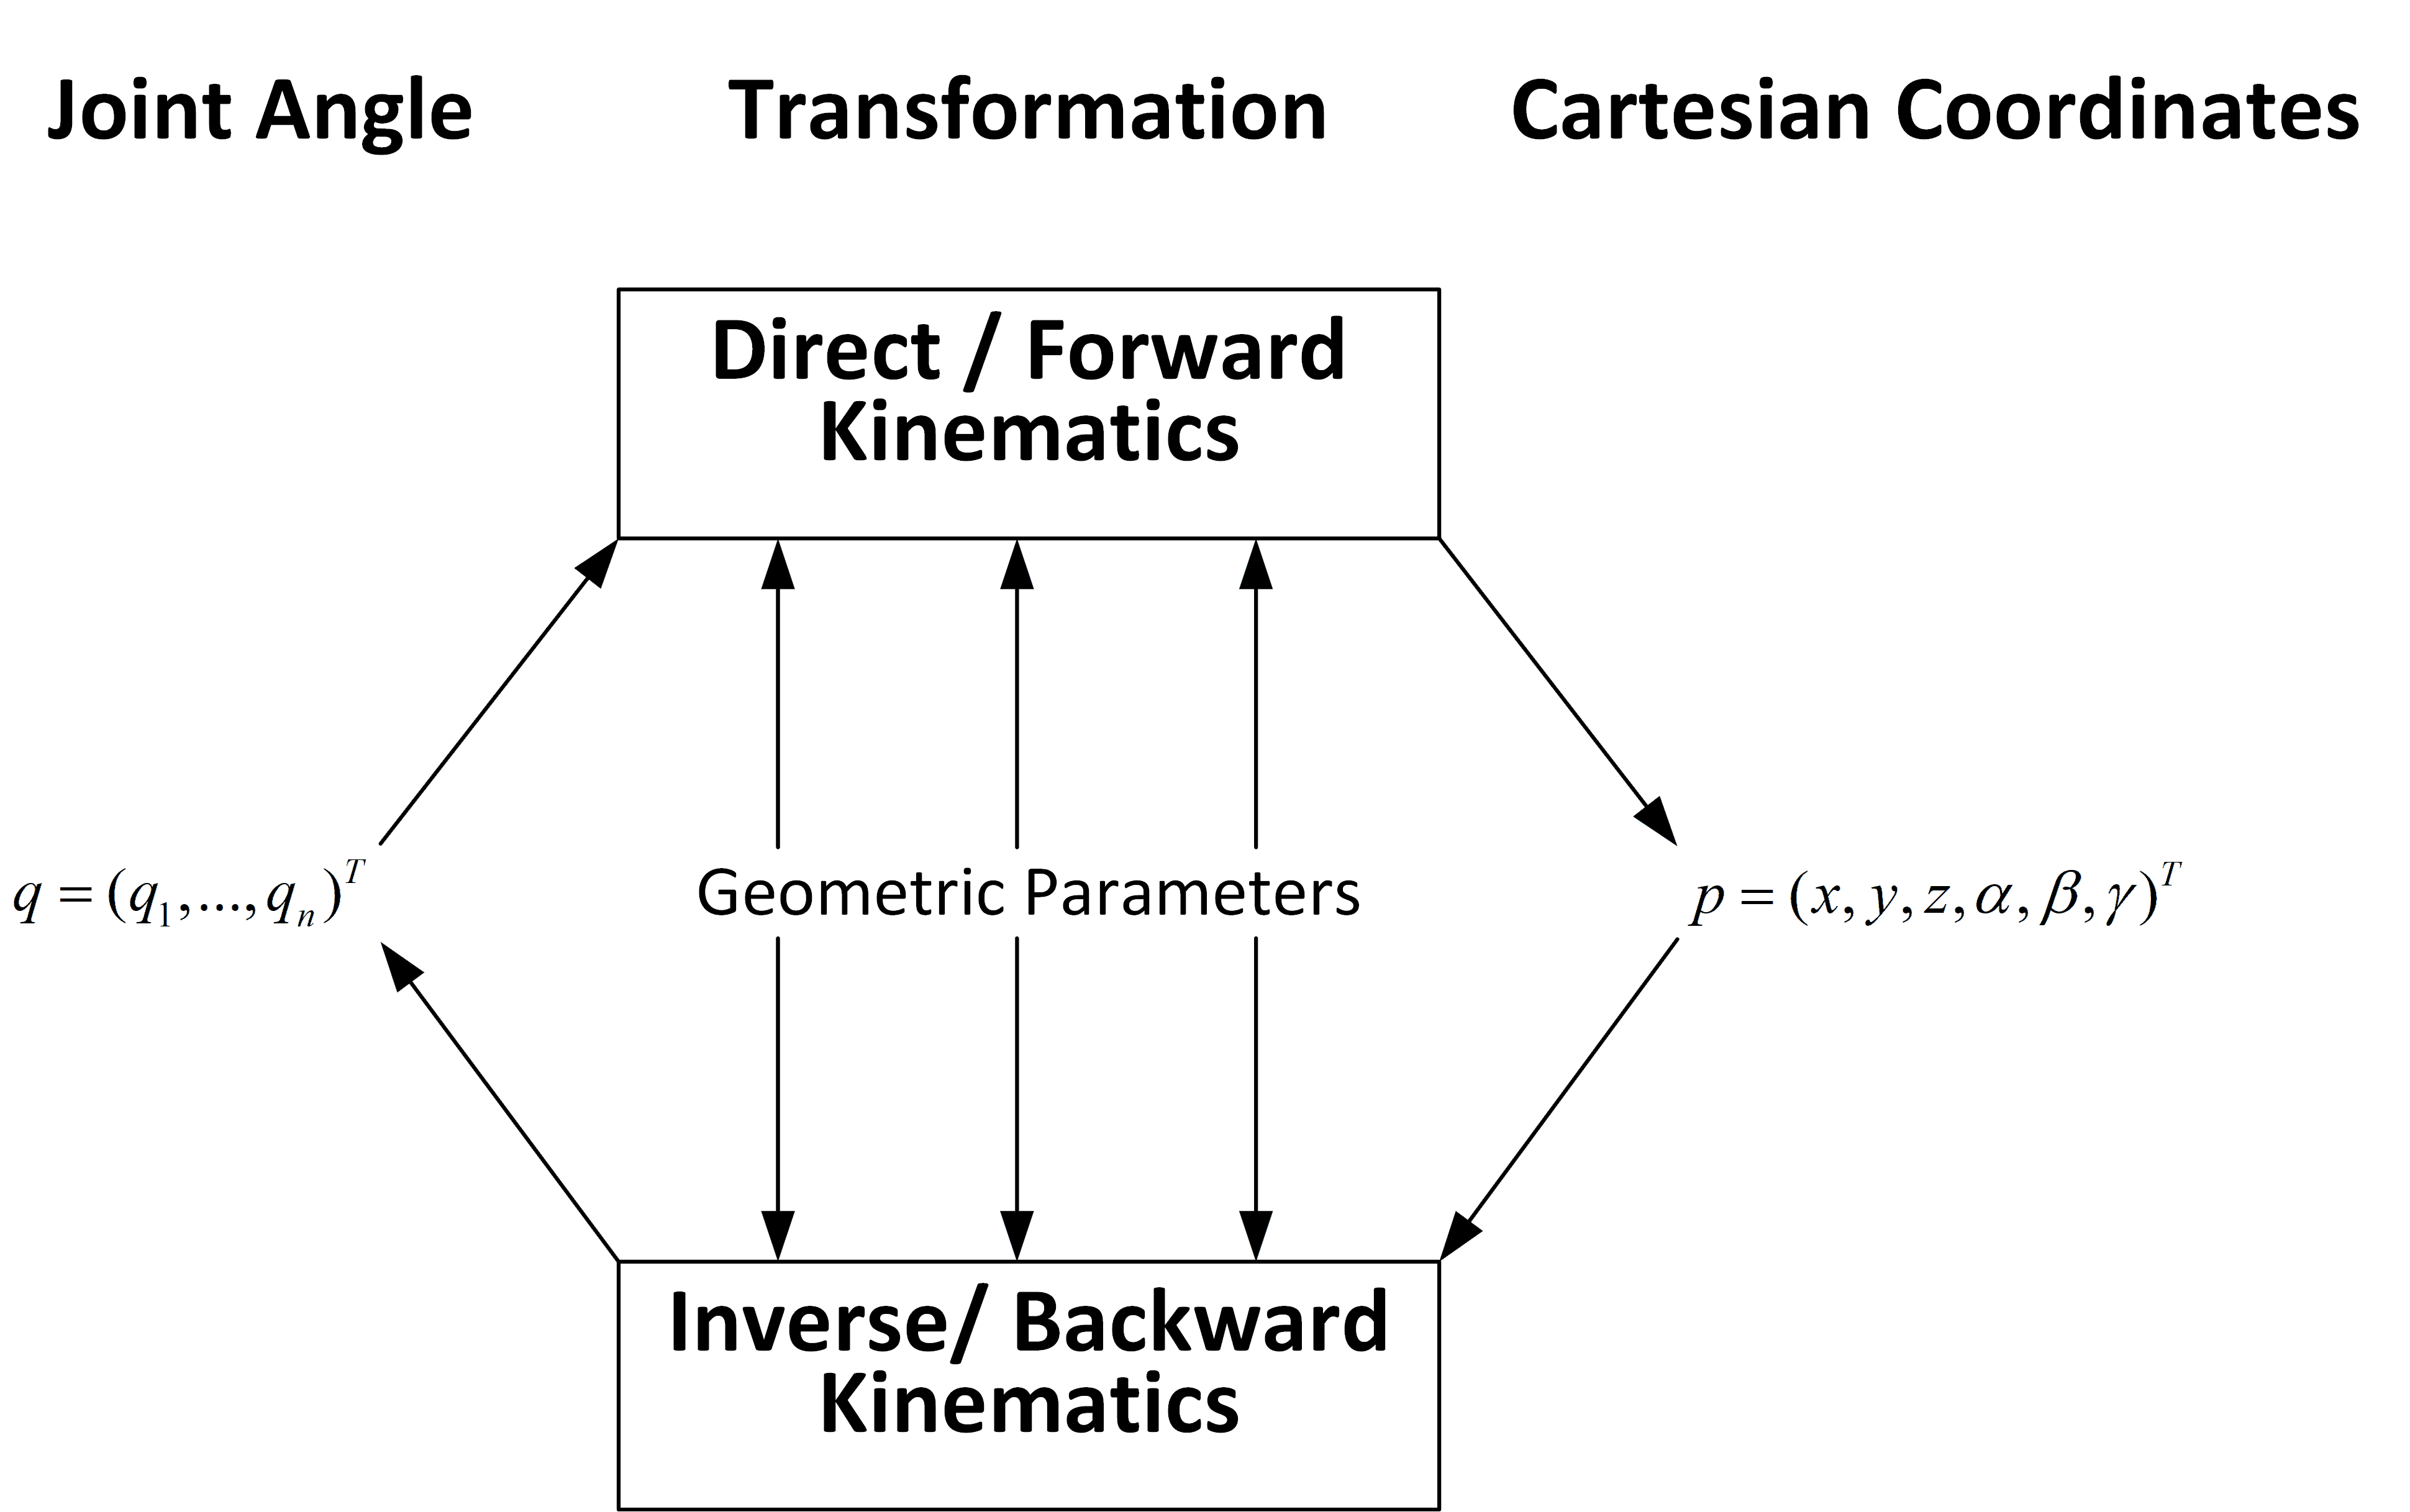
\includegraphics[
	width=0.95\linewidth,
	right,
	keepaspectratio,
	]{VisioDrawings/FWDvsINV_Kinematics_HighResTransp}
	\caption{Relation between inverse and forward kinematics translated from German Wikipedia site on inverse inematics \cite{forwardVsInverseKinematics}}
	\label{fig:FwVsInvKin}
\end{figure}

In the german wikipedia article on inverse kinematics \cite{inverseKinematikWiki}, the thesis "Verallgemeinerte inverse Kinematik für Anwendungen in der Robotersimulation und der virtuellen Realität" \cite{allgInvKin} is given as one of the main sources. 
This thesis work gives a good overview on the topic of inverse kinematics. 
As stated in this thesis work, the Denavit-Hartenberg notation is a robotic convention to map the local coordinate systems within a kinematic chain as found in robot arms.

As seen in "A Mathematical Introduction to Robotic Manipulation" \cite{MathIntroRobManip} (obtained through Semantic Scholar, search phrase: robotic convention), there are several other conventions besides the "Denavit-Hartenberg notation" used in the robotics research field like the the "product of exponentials formulation".
%Another overview on robotic conventions can be found in the Wikipedia article on robotic conventions \cite{RobConventionsWiki}. 
As most literature prefers a Denavit-Hartenberg fomulation of the kinematics (see \cite{MathIntroRobManip}), this convention will be chosen in this work as well.

Solutions for forward  kinematics are simple to obtain but solving inverse kinematics  has  been  one of  the  main  concerns  in  robot kinematics research. 
With more \ac{DOF}, solutions get more complex as non-linear equations with transcendental functions need to be solved. 
For this set of equations, no general algorithms are available.
Often algebraic, geometric and iterative methods for complex manipulators are used to find a solution to the inverse kinematic problem as stated by Tarun Pratap Singh et al. \cite{FwdInvAnalysRobManip}.

To find a suitable method for solving the inverse kinematic problem, a definition for the solution is needed:\\
\medskip
\\
\fbox{\parbox{\textwidth}{"A manipulator will be considered solvable if the joint variables can be determined by an algorithm that allows one to determine all sets of joint variables associated with a given position and orientation. [...] The algorithm should find all possible solutions" -Dr.-Ing. John Nassou\cite{invKinSeriallinkMani}}}
\bigskip

With this definition of solvability, all systems with revolute and prismatic joints with 6 \ac{DOF}  in a single series chain are solvable with the current available research. \cite{invKinSeriallinkMani}
As a quick search on HAN Quest with the search term "7 DOF inverse kinematics" suggests, there is currently onging research for the inverse kinematics problem in higher DOF manipulators with fuzzy logic as multiple articles following this approach can be found.\\
\\

As the goal is to find a suitable solution strategy for the inverse kinematic problem, it helps to map out the different types of methods.
Solution strategies can be split into two classes as stated by Dr.-Ing. John Nassou \cite{invKinSeriallinkMani}:\\
\medskip


%\parbox[t][3cm][t]{7cm}{\normalsize Closed-form solutions\\}
%\parbox[t][3cm][t]{7cm}{\normalsize Numerical solutions\\} 
%Text on two sides of the page:%https://tex.stackexchange.com/questions/107491/left-and-right-aligned-text-boxes
\fbox{\begin{minipage}[t]{0.6\textwidth}
	\textbf{{\large Closed-form solutions}}\\
	faster because analytical method\\
	will find all solutions\\
	Two approaches:\\
	\\
	\begin{minipage}[t]{0.4\textwidth}
		\textbf{{\large algebraic approach}}\\
	\end{minipage}
	\begin{minipage}[t]{0.4\textwidth}
	\begin{flushright}
	\textbf{{\large geometric approach}}\\
	\end{flushright}
\end{minipage}
\end{minipage}
\hfill
\begin{minipage}[t]{0.35\textwidth}
	\begin{flushright}
		\textbf{{\large Numerical solutions}}\\
		slower because of iterative nature\\
		not always find all solutions\\
	\end{flushright}
\end{minipage}}
\medskip

As numerical methods solve within an unknown number of operations, cannot always deliver  all solutions and depend on the users decision for accuracy, \cite{invKinSeriallinkMani} a closed-form solution will be preferred.

On HAN Quest, with the keywords "6DOF inverse kinematics" the article "Inverse Kinematics Solution and Optimization of 6DOF Handling Robot" \cite{invKinSolYanWu} can be found. This offers an  algebraic method to solve the inverse kinematic problem for 6 axis robots.
A similar approach is shown in "Forward and Inverse Kinematic Analysis of Robotic Manipulators" \cite{FwdInvAnalysRobManip}\\

As an alternative, a geometric modeling can be done as seen in "Workspace analysis and geometric modeling of 6 DOF Fanuc 200IC " \cite{geomModelingKamel}. 
A completely different approach is given in "A inverse kinematic solution of  a 6-DOF industrial robot using ANN" by using artificial neural networks \cite{invKinANNKSHITISH}.\\
%https://www.tu-chemnitz.de/informatik/KI/edu/robotik/ws2016/lecture-ik%201.pdf
%
%We will split all proposed manipulator solution strategies into two broad classes:Closed-form solutions and numerical solutions.Because of their iterative nature, numerical solutions generally are much slower than closed-form solutions and do not assure to really find all solutions.For most uses, we are not interested in the numerical approach to solve inverse kinematics.Here, we will restrict our attention to closed-form solutions.In this context, we search for solutions based on an analytic expression.
%Robots, for which a closed-form solution exists, are characterized either by having several intersecting joint axes or by having many twist angles αibe equal to0 or+/-90°.
%
With one of these methods, a solution can be found for the inverse kinematic problem.
This solution can then be verified with the robotics toolbox (Corke)

With this solution, a dynamic model of the robot can be created by attaching dynamics to the model as seen in "Control and Safety Mechanisms for a 3 DOF Manipulator with Human Interaction" \cite{KongWei} and "A mathematical introduction to Robotic Manipulation" \cite{MathIntroRobManip}. A complete example of a dynamic simulation of a 6 \ac{DOF} robot arm can be found in "Dynamic Multibody Simulation of a 6-DOF Robotic Arm" \cite{Dyn6DOFBinLi}

A controller for trajectory tracking can then be created with the model as seen in "Experimental Evaluation of Nonlinear Feedback and Feedforward Control Schemes for Manipulators" \cite{evalNonlinFeedForBackControl}

This controller could then be plugged into the real robot as stated in the "Control of a FANUC Robotic arm using MATLAB manual"  \cite{FANUCcontrolMatlab} An example of this can be found in "Modelling and analysis of a 6 DOF robotic arm manipulator" \cite{RobotModelAnalContrexampleJamshed}



\section{Digital twinning}

In the setup of the experimental PL for \ac{FRC} at the \ac{SPC} 
\ac{DT} has been chosen as one of the key technologies for “Smart manufacturing”. In the cooperation with Qing, there have been a few discrepancies on the understanding of a \ac{DT}.\\
\\
To approach this topic, the term digital twin has to be defined.
This Concept was introduced for the first time by Grieves at one of his presentations about Product Lifecycle Management in 2003 at University of Michigan as a virtual representation of what has been produced \cite{GreivesDTfirst}.
As stated by Qinglin Qi \cite{Qi2018DigitalTS}, a \ac{DT} is a high fidelity virtual model for physical objects in a digital way to simulate their behaviour. 
When looking on the Wikipedia page on digital twinning \cite{DTwikip}, a wide variety of definitions can be found. 
This shows, that the concept of the \ac{DT} is not yet clearly defined. All of these definitions have in common though, that \acp{DT} are "digital replications of living as well as nonliving entities that 
enable data to be seamlessly transmitted between the physical and virtual worlds" \cite{SaddikDTmultimconv}.\\
\\
To approach the problem form the other side, it might help to look at, what is not a digital twin.
A virtual representation of a physical object without any exchange of data is a digital model \cite{WongWhatisDT}. 
If data is fed from the physical system into the model, a digital shadow is created \cite{KRITZINGER20181016}.
Only a “bi-directional relation between a physical artefact and the set of its virtual models” \cite{SchleichDTshaping} fulfils Schleich's vision of a \ac{DT}.\\
\\
As an example, a computer aided design (CAD) model is a representation of a physical entity and it is typically used to describe the shape, dimensions and materials of a construction. This model can be a 2D or a 3D model. Only if the latest sensor data associated with a matching physical device is fed into this CAD model, it can be considered a DS. \cite{WongWhatisDT} By simulating different scenarios in a model and representing the current state of the system the DS turns into a digital twin, if decisions are made automatically fed back through an actutator into the physical entity \cite{SchleichDTshaping}.
An implementation of this data transmission can be found in "Sensor Data Transmission from a Physical Twin to a Digital Twin" \cite{AlaDTdataTransmission}.\\
\\
As the \ac{DT} is mostly used in the context of \acp{PL}, it makes sense to look for similar examples in other industries, that have undergone comparable transformations with the beginning of the digital age.
Such a comparable system can be found in the transport industry. 
\acp{PL} have several points in common with train networks.
%As in train networks, \acp{PL} often handle big masses at high velocities. As trains, the machines in a \ac{PL} run in a 
%defined environment that they cannot leave. People can get involved and cross the paths of trains or 
%machines in the case of \acp{PL}. Both train networks and \acp{PL} would ideally have full safety protection, full 
%automatization and failure recovery while delivering best performance.\\
%\\
%When looking at these similarities, it becomes obvious to base a twinning specification for production lines on an existing comparable system found in rail infrastructure.
One of the latest internationally standardized systems in rail infrastructure is \ac{ETCS} which will probably become the standard signalling and control component in all European countries. 
A great overview on the \ac{ETCS}-standard is given by Thales on their website \cite{ThalesETCS}
























%In the module Systems modelling of the master course control systems at HAN, the 4+1 approach \ref{4+1} was presented. 
%
%\begin{figure}[H]
%	\centering
%	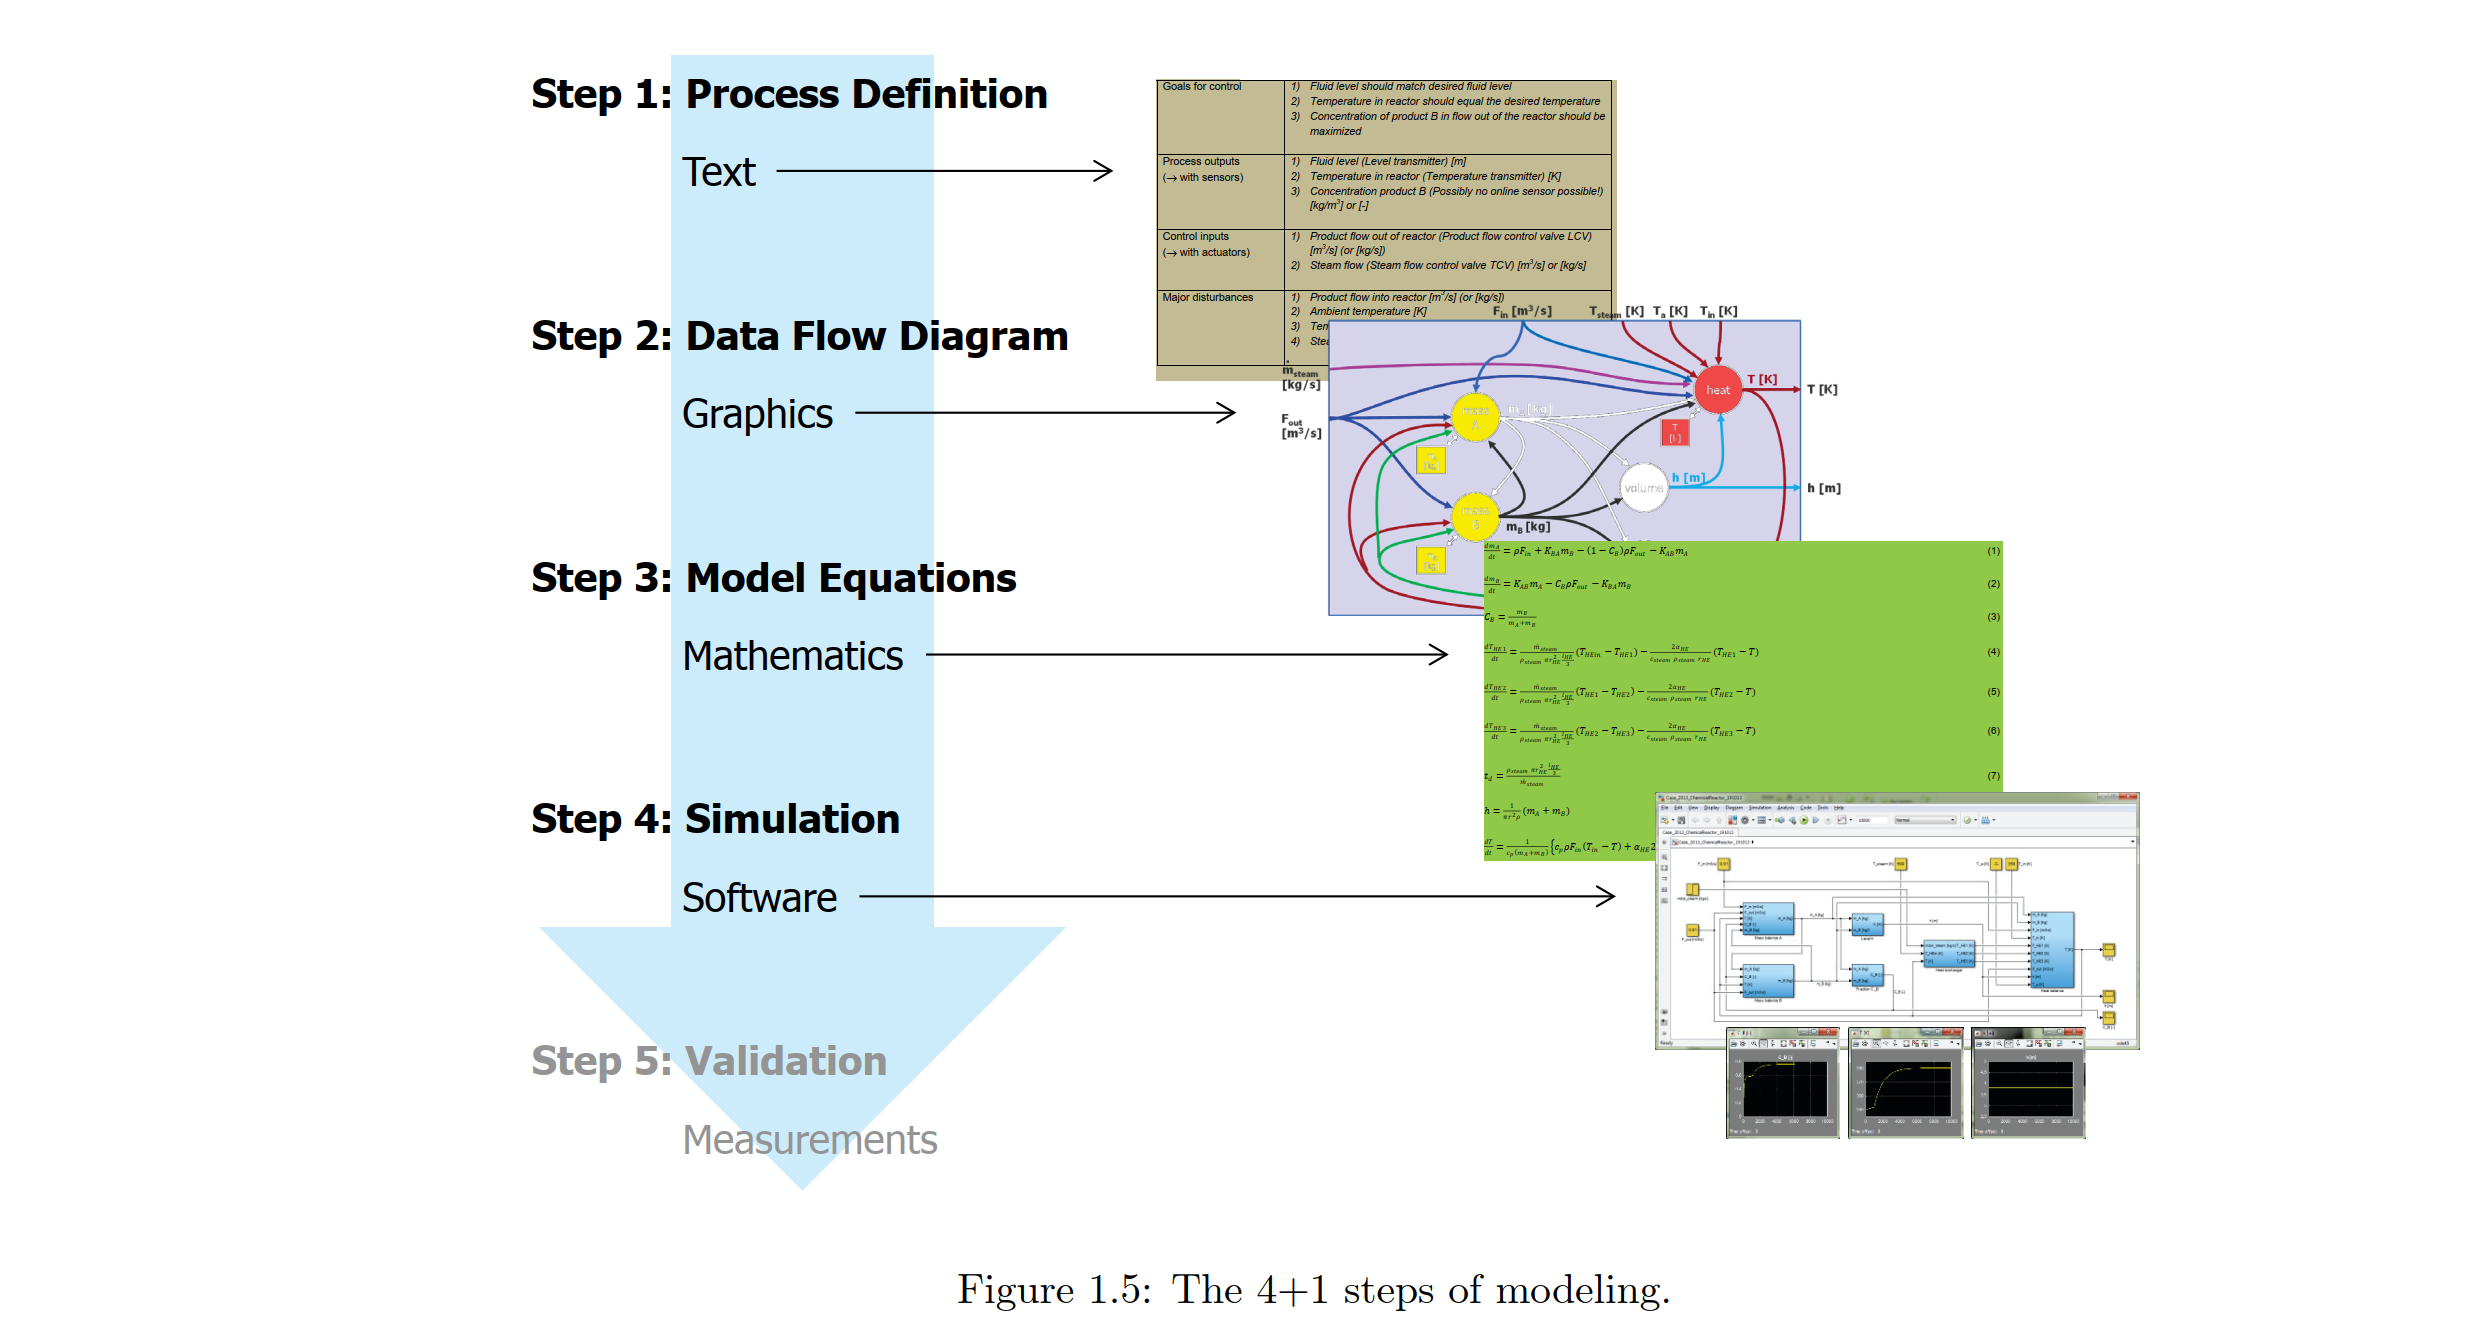
\includegraphics[
%	width=1\linewidth,
%	height=\paperheight,
%	keepaspectratio,
%	]{4+1Approach}
%	\caption{4+1 steps of modeling}
%	\label{fig:4+1}
%\end{figure}
%\pagestyle{empty}
%
%Starting from the process definition, model equations are derived with the help of a data flow diagram that lead to a simulation in software, e.g. Matlab. If possible, in the "+1" step, this model is validated with the real system.
%
%\section{Process Defintion}
%For object manipulation and other tasks, a robot arm needs to move to desired positions or track a given path. As the process focusses on the endpoint position of the robot arm, the process output can be defined as the xyz-position of the toolhead in space. The input, which can be used to control this output is the desired position. Another input that effects the output are objects attached to or carried by the robot arm. These can be considered disturbance inputs. From this, the process definition can be derived as seen in \ref{tab:ProcessDefinition}.
%
%\begin{table}[H]
%	\centering
%	\caption{Process Definiton}
%	\begin{tabular}{ll}
%		Goal for control:& Endpoint position of Robot arm   \\
%		Process output: & Endposition of Robot arm
%		 (sensor: measured with pulse encoders on the axes)   \\
%		Control inputs: & Electric power to the actuators
%		 (actuator: motor)  \\
%		Major disturbance & Carried object  
%	\end{tabular}
%\label{tab:ProcessDefinition}
%\end{table}
	
	%\chapter{Research plan}

	
	\chapter{Forward Kinematics}

To model the movements of the end effector of a kinematic chain, a forward kinematic analysis is needed. This means, that the position of the endpoint in the operational space needs to be described by the kinematic equations with the joint space as input. The non-linear kinematic equations map the joint parameters to the configuration of the robot system.   This results in a pure geometrical description of motion  by means of position, orientation, and their time derivatives.

\section{Approach}
A serial-link manipulator consists of links in a chain connected by joints. 
A link is a rigid body, defining the spatial relationship between two following axes.
For describing the serial-link mechanism geometry the Denavit Hartenberg notation is one possible approach.
It gives a description of a manipulator for kinematic solutions, Jacobians, dynamics, motion planning and simulation. 
This description can be obtained through a five step algorithm:\cite{ConstantinForwardKA}

\section{Numbering the joints and links}
A serial link robot with n joints has $n+1$ links. 

\paragraph{numbering of links}
The numbering scheme for links starts at $(0)$ with the fixed grounded base and then increases sequentially up to $(n)$ for the end effector.

\paragraph{numbering of joints}
The numbering scheme for joints starts at $(1)$ with the joint connecting the first movable link to the base and then increases sequentially up to n.

\paragraph{relation between links and joints}
Link $(i)$ is connected to its 
\begin{itemize}
	\item lower link $(i-1)$ at its proximal \cite{proxdist} end by joint $(i)$
	\item upper link $(i+1)$ at its distal \cite{proxdist} end by joint $(i+1)$
\end{itemize}

\paragraph{Joint and link numbering in Fanuc 210F}

This numbering scheme can be applied to the Fanuc 210F (see \ref{fig:LinksANDJoints210F}) 


\begin{figure}[H]
	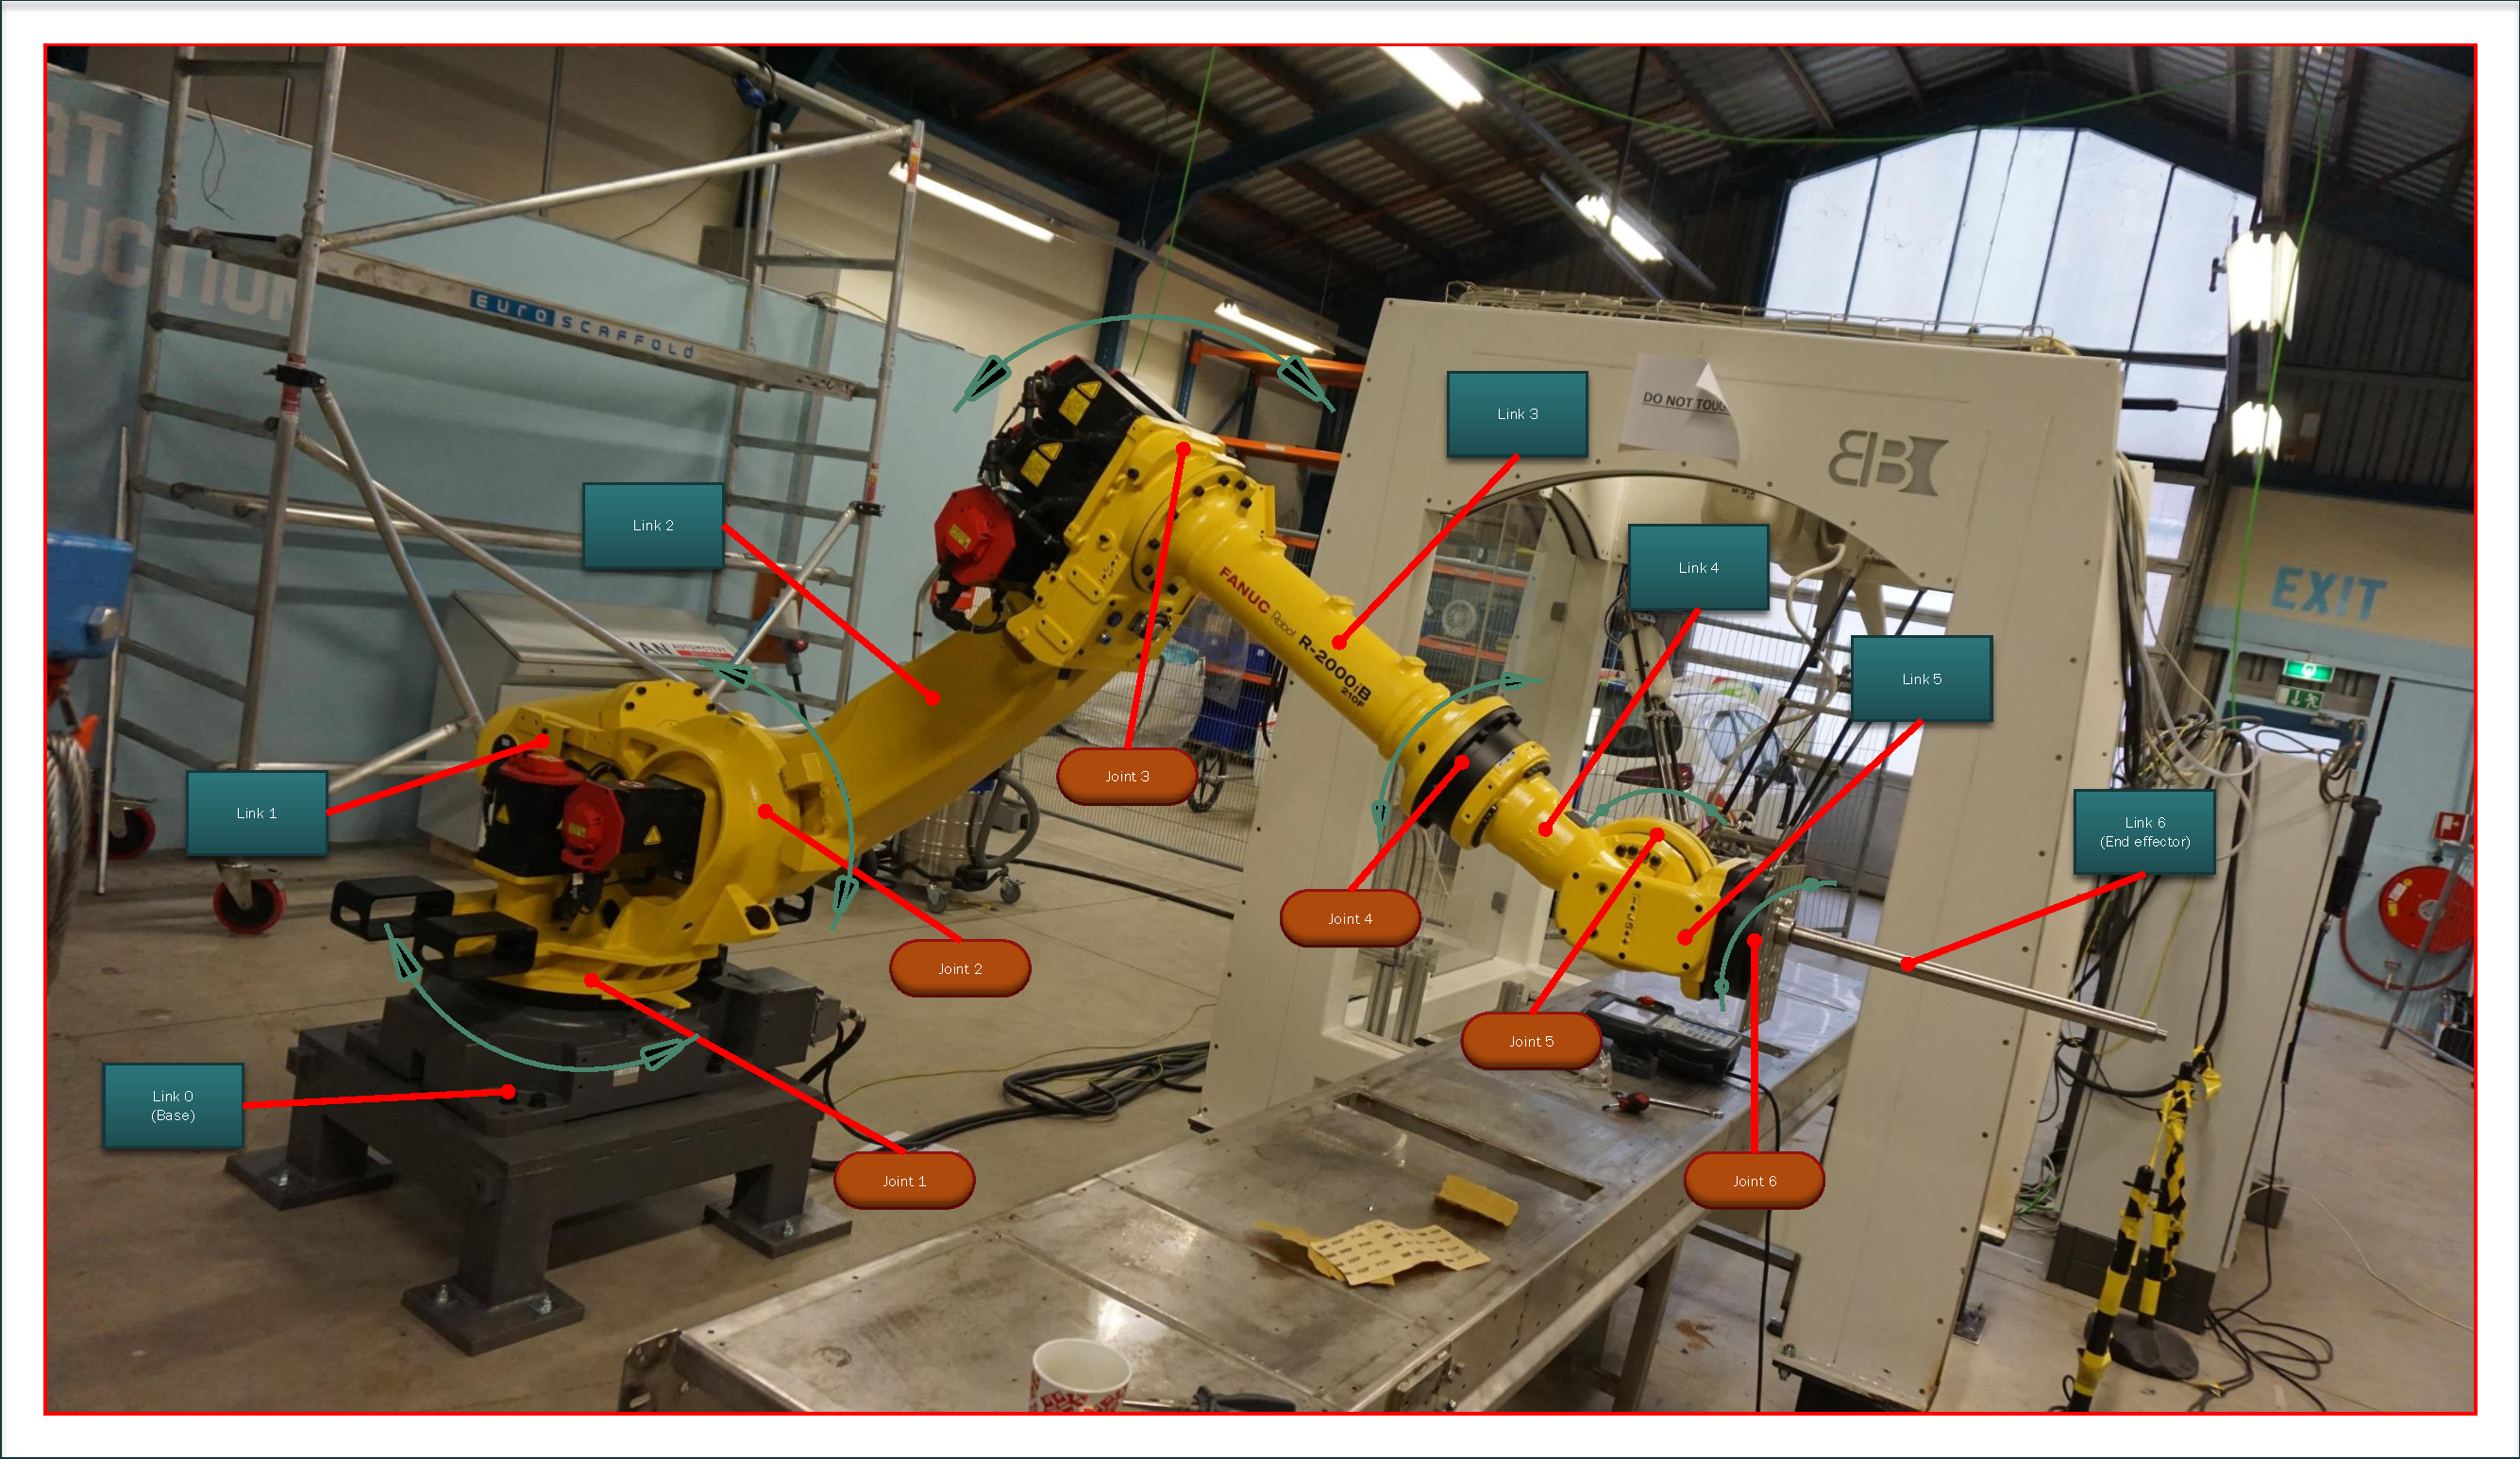
\includegraphics[
	width=1\linewidth,
	center,
	keepaspectratio,
	]{linksANDjoints/linksAndJoints}
	\caption{Links (turquoise) and joints (orange) in the FANUC 210F}
	\label{fig:LinksANDJoints210F}
\end{figure}



\section{local coordinate reference frames}
With the Denavit-Hartenberg convention, local coordinate frames can be attached to the far end of the links $ (i) $ and their accompanying joints $ (i+1) $.
Each link $(i)$ is described relative to the pose of the preceding link.

%\paragraph{Assignation of coordinate frames}


\paragraph{Assignation of $z_i$ axes}

With the DH-notation, the $z_i$ axes are assigned to link $(i)$.
Two cases need to be considered: %regarding joint $(i+1)$:
\begin{itemize}[wide=\parindent]
	\item[\textbf{revolute:}] $z_i$ is the axis of revolution of joint $(i+1)$
	\item[\textbf{prismatic:}] $z_i$ is the axis of translation of joint $(i+1)$
\end{itemize}
%of joint $(i+1)$
This means, that joint $z_i$ turns around axis $z_i$.

\paragraph{Direction of rotation}
With the direction of the $z_i$-axis, the direction of positive rotation around joint $(i+1)$ is also given by the right hand rule (see \cite{Angela_U1S2P1} at 10:35). This means, the direction of positive rotation is counter-clockwise around the $z_i$-axis.
With predictive choice of the direction of positive rotation, the direction of the z-axis can be chosen in order to minimize the DH-parameters (insert source here)

\paragraph{$z_i$ axes in Fanuc 210F}
As described above, the $z_i$ axes can be attached to the Fanuc 210F (see figure \ref{fig:zi_Axes}).


\begin{figure}[H]
	\includegraphics[
	width=1\linewidth,
	center,
	keepaspectratio,
	]{coordinateFrames/z_axes}
	\caption{$z_i$ axes on the Fanuc 210F with the direction of positive rotation (orange)}
	\label{fig:zi_Axes}
\end{figure}

The positive direction of the triples $z_1$, $z_2$, $z_4$ and $z_0$, $z_3$, $z_5$, was chosen to make sure, the x-axis would always have the same direction for parallel joints. 

\paragraph{Base frame}

The base frame $(0)$ can be chosen nearly arbitrarily. The origin of the base frame can be any point on $z_0$. For simplicity, the origin of frame$(0)$ can be put into joint$(1)$.  Usually, the x-axis of the base frame is chosen, so that it points in the direction of the \ac{EOAT} in default position according to its base, \cite{DenavitHartenbergKonventionen} but can be chosen in any convenient manner \cite{SpongDynContr}.

\paragraph{Assignation of frames $(i)$}

Starting from frame $(0)$ in an iterative process, frame $(i)$ can be set up using frame $(i-1)$.

Three cases regarding the relationship of axes $z_{i-1}$ and $z_i$  need to be considered when setting up frames:
\begin{itemize}[wide=\parindent] %option solves alignment problem for item label %https://tex.stackexchange.com/questions/246394/alignment-of-labels-in-itemize-with-text-of-document 
	\item[\textbf{Non coplanar:}] Axes don't intersect and are not parallel. Line containing the common normal $z_{i-1}$ to $z_i$ defines $x_i$-axis and the point of intersection with $z_i$ is the origin of frame $(i)$
	\begin{enumerate}[label=\emph{\alph*)}]
		\item find common normal of the joint axes
		\item put origin in intersection of normal with joint axis
		\item put $z_i$ axis in the joint axis
		\item $x_i$ points in direction of the common normal, facing away from frame $(0)$
		\item add $y_i$ according to right hand rule
	\end{enumerate}
	\item[\textbf{Parallel:}] Axes are parallel. Line containing the normal through origin of frame $(i+1)$ and the $z_i$-axis defines the $x_i$-axis which is directed from origin of frame $(i)$ toward the distal joint. The point of intersection of common normal with $z_i$-axis gives the origin of frame $(i)$. % found a mistake here with common normal in \cite{ConstantinForwardKA} witht he help of \cite{SpongDynContr}. The x-axis should point towards next joint, but he says, should point towards last joint, but does it actually the other way around.
		\begin{enumerate}[label=\emph{\alph*)}]
		\item look for normal originating from distal joint
		\item put origin in the intersection of the normal with the joint axis
		\item put the $z_i$ axis in the joint axis of the link $(i+1)$ 
		\item $x_i$ points follows the common normal with the distal joint, pointing towards the distal joint
		\item add $y_i$ according to right hand rule
	\end{enumerate}
	\item[\textbf{Intersecting:}] Axes are intersecting. Line containing the normal to the plane formed by axes $z_{i-1}$ and  $z_i$ gives the $x_i$-axis with positive direction chosen arbitrarily. Point of intersection of  axes $z_{i-1}$  and  $z_i$ is the origin of frame $(i)$.
		\begin{enumerate}[label=\emph{\alph*)}]
		\item put origin in intersection point of the axes
		\item put the $z_i$ axis in the joint axis of the link $(i+1)$
		\item $x_i$ is perpendicular to both joint axes
		\item add $y_i$ according to right hand rule
	\end{enumerate}
\end{itemize}

\paragraph{Assignation of \ac{EOAT} frame}
As there is no distal joint for the \ac{EOAT} frame, the steps for this frame are different:

\begin{enumerate}[label=\emph{\alph*)}]
	\item put origin on axis of proximal joint 
	\item axis $z_i$ follows direction of $z_{i-1}$
	\item $x_i$ can be chosen arbitrarily, but is usually determined by screw holes
	\item add $y_i$ according to right hand rule
\end{enumerate}

\paragraph{local coordinate reference frames on the Fanuc 210F}

As described above, the local coordinate reference frames can also be attached to the Fanuc 210F as seen in \ref{fig:RefFrame}. 

\begin{figure}[h]
	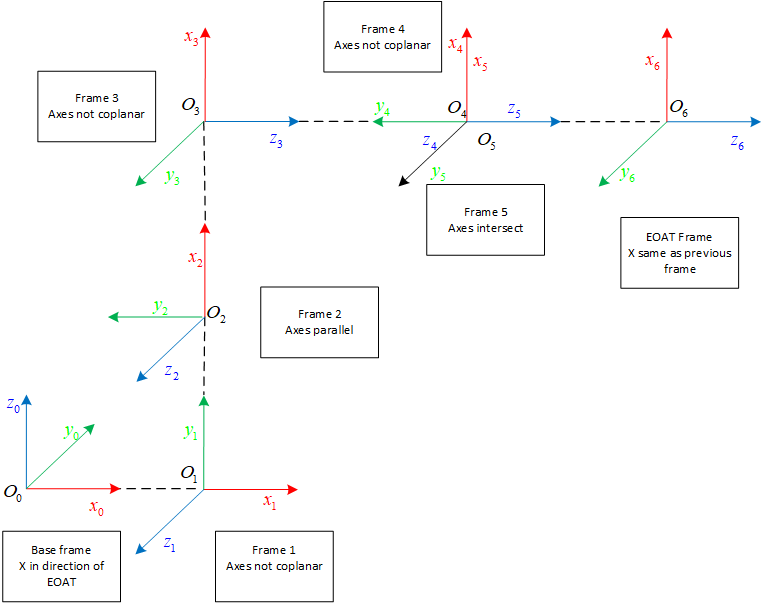
\includegraphics[
	width=1\linewidth,
	center,
	keepaspectratio,
	]{coordinateFrames/CoordinateFrames}
	\caption{Coordinate reference frames for Fanuc 210F}
	\label{fig:RefFrame}
\end{figure}

\paragraph{frame 0 (Base)}
The frame mapping starts with the base frame. For the base frame the z-axis is given through joint $j_1$. Origin of frame 0 is put into joint 1.
The x-axis is chosen to point in direction of of the \ac{EOAT} in standard pose. For standard pose see \ref{fig:StandardPose}.
This pose will also be chosen for alignment of all distal frames.

\begin{figure}[h]
	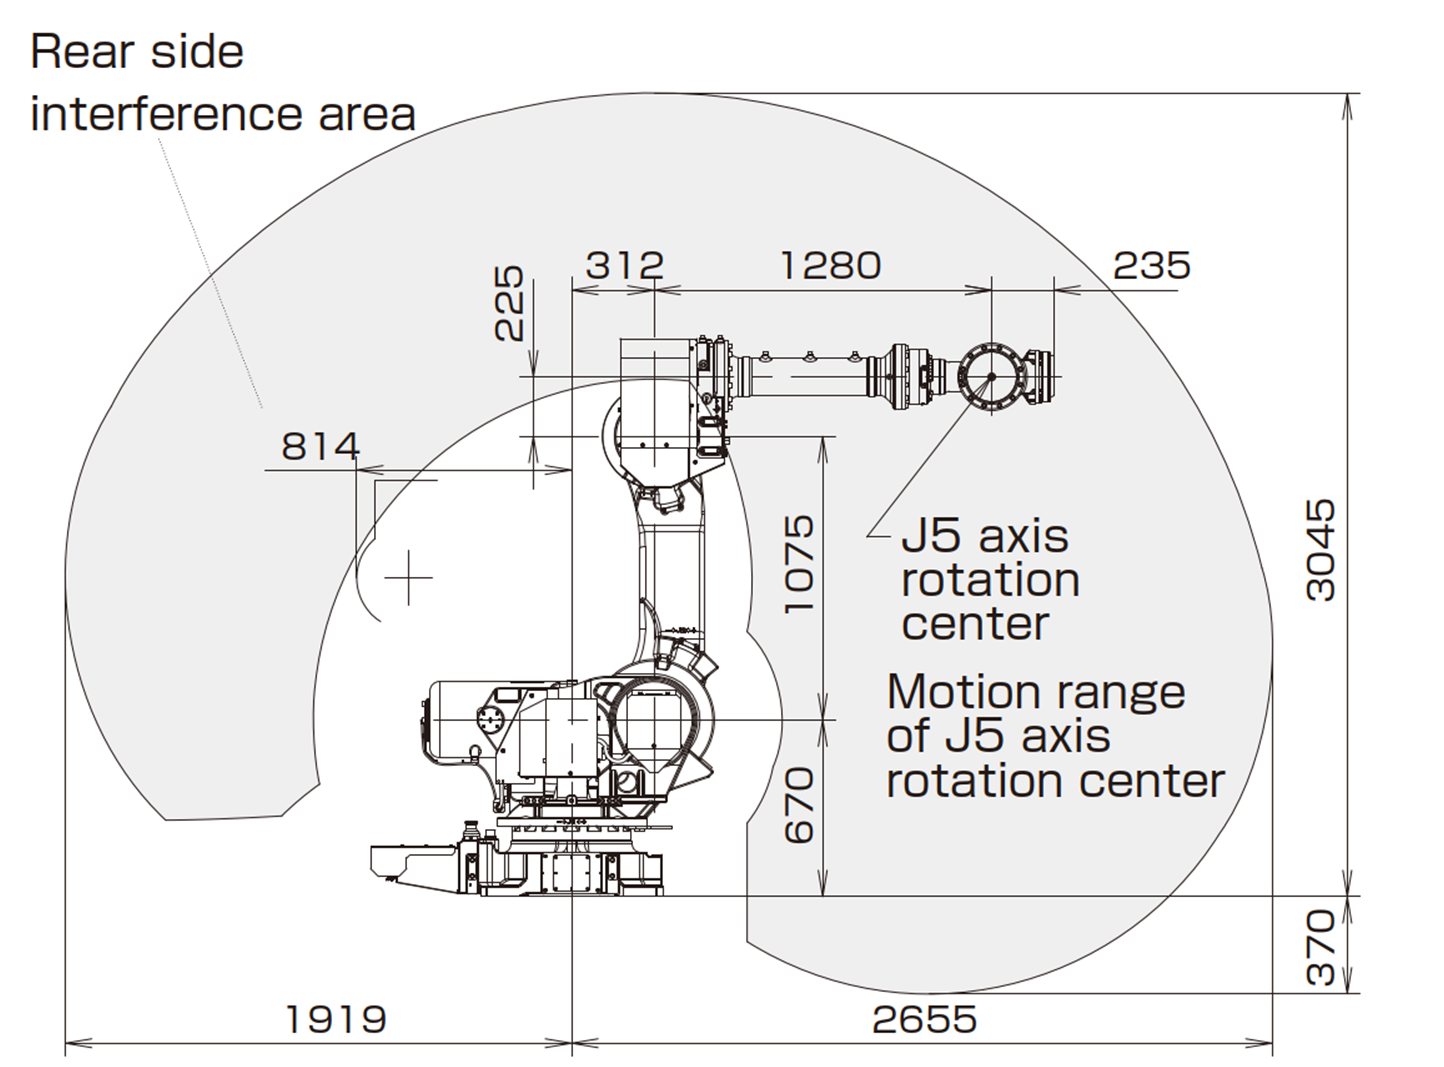
\includegraphics[
	width=1\linewidth,
	center,
	keepaspectratio,
	]{coordinateFrames/standardPose}
	\caption{Standard pose of the robot}
	\label{fig:StandardPose}
\end{figure}

\paragraph{frame 1}
For frame 1, the z-axes are not coplanar. 
Because of that, the  $z_0$-axis is extended until a common normal can be found that intersects with $z_i$ to define the origin $O_1$.
$x_1$ departs from $O_1$ along the common normal.
$y_1$ is added according to the right hand rule.

\paragraph{frame 2}
As seen, in image \ref{fig:zi_Axes}, axes $z_2$ and $z_1$ are parallel. $O_2$ can be found at the intersection of the normal through $O_1$ with $z_2$. $x_2$ follows the common normal with joint 4.
$y_2$ is added according to the right hand rule.

\paragraph{frame 3}
Joint 3 and joint 4 are not exactly aligned (see image \ref{fig:StandardPose}), which prevents the z-axes to intersect. That's why axes $z_3$ and $z_2$ are not coplanar. 
$z_3$ runs parallel through the link 3, due to the orientation of the rotational axis.
As the common normal between $z_3$ and $z_2$ defines $x_3$, which in turn gives $O_3$, the origin can be found far away from the physical position of the joint.
$y_3$ is added according to the right hand rule.

\paragraph{frame 4}
Joint 5 lies in line with joint 4.
As $z_3$ follows this line, the axes  $z_4$ and $z_3$ intersect in the center of joint 5, which gives $O_4$. 
$x_4$ leaves the plane spanned by  $z_4$ and $z_3$ perpendicular.
The positive direction of $x_4$ is chosen to be similar as in frame 3 for simplicity.
$y_4$ is added according to the right hand rule and points in direction of frame 3.

\paragraph{frame 5}
As $z_5$ lies  in line with $O_4$, the axes  $z_5$ and $z_4$ intersect in $O_4$ which puts $O_5$ at the same position as $O_4$.
$x_5$ leaves the plane spanned by  $z_5$ and $z_4$ perpendicular.
The positive direction of $x_5$ is chosen to be similar as in frame 4 for simplicity, which puts $x_5$ and $x_4$ on top of each other. 
$y_5$ is added according to the right hand rule and as $z_5$ is turned 90 degrees relative to $z_4$ around $x_{4,5}$, $y_5$ is turned 90 degrees relative to $z_4$ around $x_{4,5}$ as well.

\paragraph{frame 6 (EOAT)}
$z_6$ lies in line with $z_5$ and is consequently parallel.
as there are no distal joints, to reference $x_6$, it can be chosen arbitrarily. 
For simplicity, it is chosen to be similar as in frame 5. 
$y_6$ is added according to the right hand rule.

\section{Establishing \ac{DH} parameters for each link}

After assigning the local coordinate frames, the \ac{DH}-Transformations have to be determined. This leads to a kinematic chain with each frame determined by the previous one \cite{DenavitHartenbergKonventionen}.

Link0 - Link1 - Link2 - Link3 - Link4 - Link5 - Link6

Each \ac{DH}-transformation consists of four elementary transformations\cite{DenavitHartenbergKonventionen}:

\begin{enumerate}[label=\emph{\arabic*)}]
	\item rotation around the $x_i$-axis with the amount of $\alpha_i$
	\item translation along $x_i$-axis with the amount of  $a_i$
	\item translation along $z_i$-axis with the amount of  $d_i$
	\item rotation around $z_i$-axis with the amount of  $\theta_i$
\end{enumerate}

This shows that the \ac{DH} robotic convention is a minimal line representation, as with four parameters, all possible lines in the Euclidean Space can be represented (\cite{AutRobVeh}, page 210).

Following from this, two pairs of parameters determine the joints and links \cite{ConstantinForwardKA}:
\begin{itemize}[wide=\parindent] 
	\item[Links:] represented by link length ($a$) and link twist ($\alpha$)
	%, defined as the relative location of the two attached joint axes.
	\item[Joints:] represented by link offset ($d$)
	% which is the distance from one link to the next 
	and joint angle ($\theta$) 
	%which is the rotation of one link with respect to the next around the joint axis.
\end{itemize}

These are the \ac{DH}-parameters which form the transformation matrices that connect serial link coordinate frames. They can be distinguished into parameters and variables. While constructive parameters are dependent on the construction of the robot and are constant, variables depend on the joint movement \cite{FwdInvAnalysRobManip} \cite{ConstantinForwardKA} \cite{DenavitHartenbergKonventionen}.

\begin{enumerate}[label=\emph{\arabic*)}]
	\item[$\alpha_i$] angle between $z_{i-1}$ and $z_i$, measured in plane normal to $x_i$ (constructive parameter)
	\item[$a_i$] distance between $z_{i-1}$ and $z_i$, measured along $x_i$; parallel to $z_{i-1} \times z_i$ for intersecting axes (constructive parameter)
	\item[$d_i$] distance from the origin $O_{i-1}$ of frame $i-1$ to the intersection of the $x_i$ axis with $z_{i-1}$, measured along $z_{i-1}$ (constructive parameter in revolute joints, variable in prismatic joints)
	\item[$\theta_i$] angle between $x_{i-1}$ and $x_i$, measured in plane normal to $z_{i-1}$ (constructive parameter in prismatic joints, variable in revolute joints)
\end{enumerate}

These parameters describe the relatively complex transformation of the coordinate system $i-1$ into the coordinate system $i$ by four subsequent elementary transformations \cite{allgInvKin}:

\begin{equation} \label{eq:DH-Transform}
	T_{i-1,i}=ROT(z_{i-1}, \theta_i) * TRANS(0,0,d_i)^T * TRANS(a_i,0,0)^T * ROT(x_i,\alpha_i)
\end{equation}

$ROT(v,\alpha)$ is a simple rotation around vector $v$ with the angle $\alpha$ and $TRANS(x,y,z)^T$ is a translational movement along the vector $[x,y,z]^T$. For a visual representation of these parameters see figure \ref{fig:DH_Parameters_visual} 

\begin{figure}[H]
	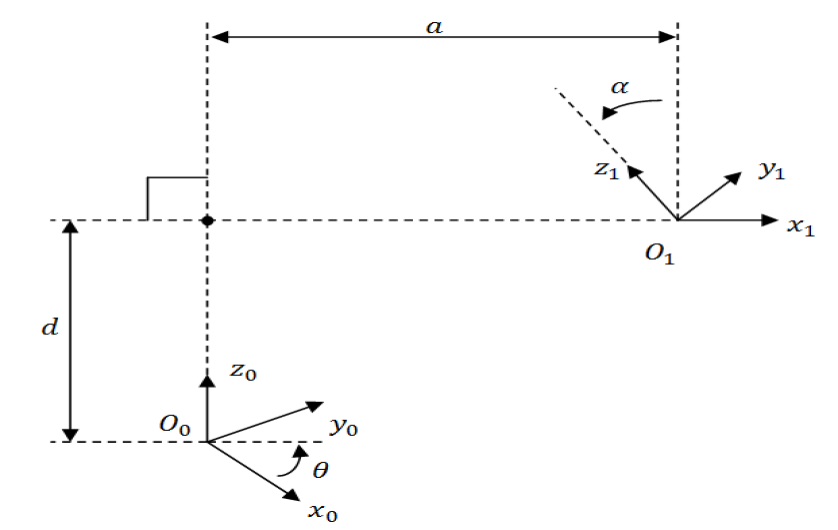
\includegraphics[
	width=0.8\linewidth,
	center,
	keepaspectratio,
	]{coordinateFrames/DH_Parameters_visual}
	\caption{Visual representation of a \ac{DH}-transformation}
	\label{fig:DH_Parameters_visual}
\end{figure}

This visual representation gives a guide to attach the \ac{DH}-parameters on serial-link mechanisms.


\section{Establishing \ac{DH} parameters on the Fanuc 210F}

As described above, the \ac{DH}-Parameters can also be determined for the Fanuc 210F.
These parameters can be found with the help of the assigned coordinate frames as seen in figure \ref{fig:DH_Parameters_Fanuc210F}. For simplicity, only non-zero DH-parameters are shown in this figure.

\begin{figure}[H]
	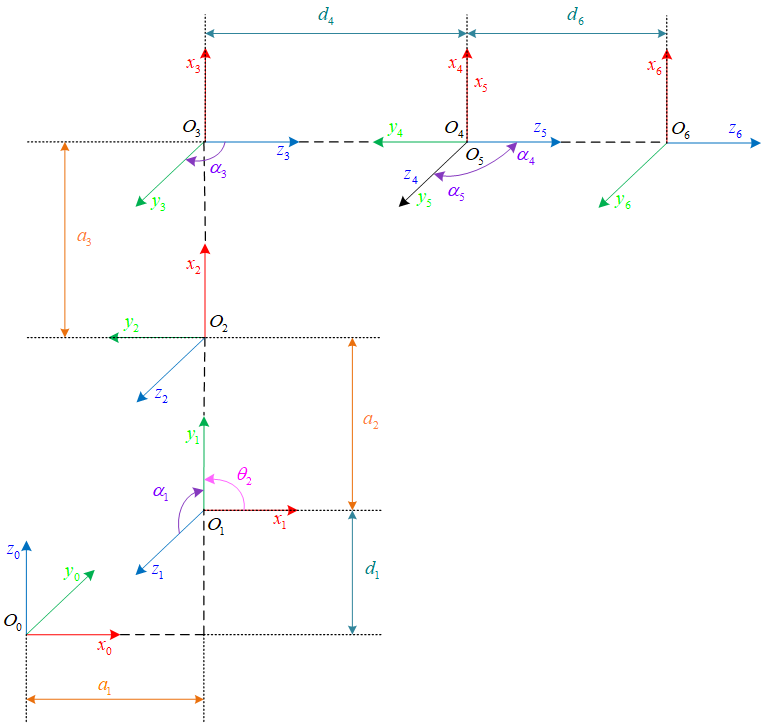
\includegraphics[
	width=1\linewidth,
	center,
	keepaspectratio,
	]{coordinateFrames/DH_Parameters_assignment}
	\caption{Assignment of DH-Parameters on the Fanuc 210F}
	\label{fig:DH_Parameters_Fanuc210F}
\end{figure}


To wrap this up, a summary of the D-H parameters for each link as follows from figure \ref{fig:DH_Parameters_Fanuc210F} can be found in table \ref{table:DH-Parameter}


%Generate tables easily with: % https://www.tablesgenerator.com/

	\begin{table}[H]
		\centering
	\begin{tabular*}{0.5\textwidth}{|l||@{\extracolsep{\fill}}l|l|l|l|}
		\hline
		Link & \multicolumn{1}{l|}{$\theta_i$} & \multicolumn{1}{l|}{$d_i$} & \multicolumn{1}{l|}{$a_i$} & \multicolumn{1}{l|}{$\alpha_i$} \\ \hline\hline
		1 & $\theta_1$ & $d_1$ & $a_1$ & $\alpha_1$\\ \cline{1-5}
		2 & $\theta_2$ & 0     & $a_2$ & 0         \\ \cline{1-5}
		3 & $\theta_3$ & 0     & $a_3$ & $\alpha_3$\\ \cline{1-5}
		4 & $\theta_4$ & $d_4$ & 0     & $\alpha_4$\\ \cline{1-5}
		5 & $\theta_5$ & 0     & 0     & $\alpha_5$\\ \cline{1-5}
		6 & $\theta_6$ & $d_6$ & 0     & 0         \\ \cline{1-5}
		%\hline
	\end{tabular*}
\caption{Denavit Hartenberg Parameters for Fanuc 210F}
\label{table:DH-Parameter}
\end{table}

\section{numeric values of DH-Parameters}

As can be seen from table \ref{table:DH-Parameter}, many \ac{DH}-parameters are zero due to a good choice of pose and coordinate frames. 
All angles are plus or minus 90°.
 
Most of the frames have translational transformations in either $a_i$ or $d_i$ direction with link 1 and 5 being the exception.
By lifting the base frame out of the joint, parameter $d_1$ could be set to zero as well. For better understanding, the origin of the frame was originally kept inside the joint.
Frame 5 shares the origin with frame 4, not requiring any translational movement.
Most of the frames are also rotated by 90 degree around the x-axis with link 2 and 6 being the exception. Frame 6 was chosen with the same orientation as frame 5. Frame 2 has the same x-axis orientation as link 1 because joints two and three are parallel. There is just a rotational transformation around the z-axis of 90°. This is only due to the standard pose of the robot, as theta is a variable.
For all coordinate frames theta is a variable, as all joints are revolute and none is translational. 

Besides the angle values for $\alpha_i$ which were easy to determine from the graphical interpretation in figure \ref{fig:DH_Parameters_Fanuc210F}, following numeric values need to be determined through measurements or CAD-Drawings:
$d_1$, $d_4$, $d_6$ and \\
$a_1$, $a_2$, $a_3$. 

A great help to determine these values is fig \ref{fig:StandardPose}. This technical drawing was obtained from the datasheet for all Fanuc R-2000iB series robots. 
With this drawing, following \ac{DH}-parametes can be obtained:

\begin{itemize}\label{item:DH-LinparamValues}
	\item[$a_1$=] 312mm
	\item[$a_2$=] 1075mm
	\item[$a_3$=] 225mm
	\item[$d_4$=] 1280mm
	\item[$d_6$=] 235mm
\end{itemize}

The parameter $d_1$ cannot be determined from this drawing. It can either be measured on the actual robot, or defined as zero, as frame zero can be freely moved along the z-axis. A value of zero would put the origin of the base frame on the same height as frame 1, simplifying subsequent steps. 
It must be clear though, that all referencing in the forward and backward kinematics will be relative to this point. 
A change of this point of reference can be added later simply by adding another transformation matrix for translational movement along the z-axis as presented by Richard P. Paul \cite{Paul1981RobotM}.\\
\\
This results in a table of numeric DH-parameters as seen in \ref{table:DH-Parameter_num}. The transformation $^{i-1}T_i$ depends only on a single variable $\theta_i$ as all of the other quantities stay constant, and all joints are revolute.

	\begin{table}[H]
	\centering
	\begin{tabular*}{0.5\textwidth}{|l||@{\extracolsep{\fill}}l|l|l|l|}
		\hline
		Link & \multicolumn{1}{l|}{$\theta_i$} & \multicolumn{1}{l|}{$d_i$} & \multicolumn{1}{l|}{$a_i$} & \multicolumn{1}{l|}{$\alpha_i$} \\ \hline\hline
		1 & $\theta_1$ & 0     & 312   & $\pi/2$  \\ \cline{1-5}
		2 & $\theta_2$ & 0     & 1075  & 0        \\ \cline{1-5}
		3 & $\theta_3$ & 0     & 225   & $\pi/2$  \\ \cline{1-5}
		4 & $\theta_4$ & 1280  & 0     & $-\pi/2$ \\ \cline{1-5}
		5 & $\theta_5$ & 0     & 0     & $\pi/2$  \\ \cline{1-5}
		6 & $\theta_6$ & 235   & 0     & 0        \\ \cline{1-5}
		%\hline
	\end{tabular*}
	\caption{Numeric values of Denavit Hartenberg Parameters for Fanuc 210F}
	\label{table:DH-Parameter_num}
\end{table}

\section{Homogeneous transformation matrices}

Locating reference frame $(i-1)$ relative to $(i)$ can be done by executing a series of transformations as given by equation \ref{eq:DH-Transform}. 
For simplification, they can be done with a 4 × 4 homogenous transformation matrix:
\begin{equation} \label{eq:fourTransformations}
	^{i-1}T_i(\theta_i,d_i,a_i,\alpha_i)=R_z(\theta_i)*T_z(d_i)*T_x(a_i)*R_x(\alpha_i)
\end{equation}
Equation \ref{eq:fourTransformations} can be expanded into:
\begin{equation}\label{eq:TransformationMarix}
	^{i-1}T_i=
	\begin{bmatrix}
	\cos\theta_i & -\sin\theta_i*\cos\alpha_i & \sin\theta_i*\sin\alpha_i & a_i*\cos\theta_i \\
	\sin\theta_i & \cos\theta_i*\cos\alpha_i & -\cos\theta_i*\sin\alpha_i & a_i*\sin\theta_i \\ %Typo in source column 3 - source used cos instead of sin alpha_i
	0 & \sin\alpha_i & \cos\alpha_i & d_i \\
	0 & 0 & 0 & 1 \\
	\end{bmatrix}
\end{equation}

For further details on how to set up $R_z(\theta_i), T_z(d_i), T_x(a_i) and R_x(\alpha_i)$ and form the transformation matrix in equation \ref{eq:TransformationMarix} see chapter one "HOMOGENEOUS TRANSFORMATIONS" in "Robot manipulators: mathematics, programming, 
and control: the computer control of robot manipulators" \cite{Paul1981RobotM}. The basic techniques for setting up the translation and rotation matrices as well as how to combine them are described in that chapter .

\section{Forward Kinematic Equations} \label{ForKinEq}
In Forward kinematics, the kinematic equations of a robot are used to compute the position of the \ac{EOAT} from the given joint parameters.

\paragraph{Sum of Transformations Matrix}
With the transformation matrices from frame $(i)$ to $(i-1$), a $4×4$ matrix for all joints on n links can be established as in equation \ref{eq:SummofTranfMatr}

\begin{equation} \label{eq:SummofTranfMatr}
	^0T_n=\prod_{n}^{i=1} \phantom{.}^{i-1}T_i
\end{equation}


The resulting matrix has the form (see \cite{invKinSolYanWu}, eq 1):
\begin{equation}\label{eq:matrixForm}
	^0T_n=
	\begin{bmatrix}
	n & o & a & p \\
	0 & 0 & 0 & 1 \\
	\end{bmatrix}
	=
	\begin{bmatrix}
	n_x & o_x & a_x & p_x \\
	n_y & o_y & a_y & p_y \\ %mistake here in source?\cite{invKinSolYanWu} xyz broken? - error confirmed!
	n_z & o_z & a_z & p_z \\
	0 & 0 & 0 & 1 \\
	\end{bmatrix}
\end{equation}

\paragraph{short notation}
The short notations for orientation, rotation and position are defined as:

\begin{itemize}
	\item[n] normal vector
	\item[o] orientation vector
	\item[a] approach vector
	\item[p] position
\end{itemize}
  

\paragraph{Transformation to cartesian coordinates with euler angles }
These vectors can be transformed into the $[x,y,z,\alpha,\beta,\gamma]$ notation.
Vector $p = [p_x, p_y, p_z] $ gives [x, y,z].
The rotational approach $[\alpha, \beta, \gamma]$ can be calculated with the rotation matrix R as seen in eq \ref{eq:rotMatrix_composition}.
\begin{equation}\label{eq:rotMatrix_composition}
	T = 
	\begin{bmatrix}
	R & p \\
	0 & 1 \\
	\end{bmatrix}
\end{equation}

The rotation matrix describes the relative orientation of two frames towards each other. As the columns $[n,o,a]$ are the unit vectors along the axes of one frame relative to the other reference frame, the relative orientation of a frame ${b}$ with respect to a frame ${a}$ is given by the rotation matrix as seen in eq \ref{eq:rotMatrix_a-b} \cite{ConstantinForwardKA}
\begin{equation}
	\phantom{}^b_aR =
	\begin{bmatrix}
	\phantom{}_ax^b) & \phantom{}_ay^b) & \phantom{}_az^b) \\
	\end{bmatrix}
	=
	\begin{bmatrix}
	x^b \cdot x^a & y^b \cdot x^a & z^b \cdot x^a \\
	x^b \cdot y^a & y^b \cdot y^a & z^b \cdot y^a \\
	x^b \cdot z^a & y^b \cdot z^a & z^b \cdot z^a \\
	\end{bmatrix}
\end{equation}

As in equation \ref{eq:rotMatrixToAbsFrame} the coordinates relative to the reference frame ${a}$, of a point $p$, of which the coordinates are known with respect to a frame ${b}$ with the same origin can then be calculated ( see \cite{RobotKinemDyn}, "Description of Position and Orientation) .
\begin{equation}\label{eq:rotMatrixToAbsFrame}
	\phantom{}_a p = \phantom{}^b_aR\phantom{.}_b p 
\end{equation}




\section{Forward Kinematic Equations on the 210F}
As shown in fig.\ref{fig:zi_Axes}, the Fanuc 210F is a 6-\ac{DOF} robotic arm with n=six revolute joints in series. 
Their orientation can be expressed in short form with 
\begin{equation}
	(R\perp R\parallel R\perp R\perp R\perp R )
\end{equation}

With this, the complete transformation matrix can be derived in the form as described in \ref{ForKinEq}:

%\begin{equation}
\begin{multline}\label{eq:TransformMatrices_0-6}
	^0T_6=\\
	\begin{bmatrix}
\cos\theta_1 & -\sin\theta_1  \cos\alpha_1 & \sin\theta_1  \sin\alpha_1 & a_1  \cos\theta_1 \\
\sin\theta_1 & \cos\theta_1  \cos\alpha_1 & -\cos\theta_1  \sin\alpha_1 & a_1  \sin\theta_1 \\
0 & \sin\alpha_1 & \cos\alpha_1 & d_1 \\
0 & 0 & 0 & 1 \\
\end{bmatrix}
  \\
\begin{bmatrix}
\cos\theta_2 & -\sin\theta_2  \cos\alpha_2 & \sin\theta_2  \sin\alpha_2 & a_2  \cos\theta_2 \\
\sin\theta_2 & \cos\theta_2  \cos\alpha_2 & -\cos\theta_2  \sin\alpha_2 & a_2  \sin\theta_2 \\
0 & \sin\alpha_2 & \cos\alpha_2 & d_2 \\
0 & 0 & 0 & 1 \\
\end{bmatrix}
  \\
\begin{bmatrix}
\cos\theta_3 & -\sin\theta_3  \cos\alpha_3 & \sin\theta_3  \sin\alpha_3 & a_3  \cos\theta_3 \\
\sin\theta_3 & \cos\theta_3  \cos\alpha_3 & -\cos\theta_3  \sin\alpha_3 & a_3  \sin\theta_3 \\
0 & \sin\alpha_3 & \cos\alpha_3 & d_3 \\
0 & 0 & 0 & 1 \\
\end{bmatrix}
  \\
\begin{bmatrix}
\cos\theta_4 & -\sin\theta_4  \cos\alpha_4 & \sin\theta_4  \sin\alpha_4 & a_4  \cos\theta_4 \\
\sin\theta_4 & \cos\theta_4  \cos\alpha_4 & -\cos\theta_4  \sin\alpha_4 & a_4  \sin\theta_4 \\
0 & \sin\alpha_4 & \cos\alpha_4 & d_4 \\
0 & 0 & 0 & 1 \\
\end{bmatrix}
  \\
\begin{bmatrix}
\cos\theta_5 & -\sin\theta_5  \cos\alpha_5 & \sin\theta_5  \sin\alpha_5 & a_5  \cos\theta_5 \\
\sin\theta_5 & \cos\theta_5  \cos\alpha_5 & -\cos\theta_5  \sin\alpha_5 & a_5  \sin\theta_5 \\
0 & \sin\alpha_5 & \cos\alpha_5 & d_5 \\
0 & 0 & 0 & 1 \\
\end{bmatrix}
  \\
\begin{bmatrix}
\cos\theta_6 & -\sin\theta_6  \cos\alpha_6 & \sin\theta_6  \sin\alpha_6 & a_6  \cos\theta_6 \\
\sin\theta_6 & \cos\theta_6  \cos\alpha_6 & -\cos\theta_6  \sin\alpha_6 & a_6  \sin\theta_6 \\
0 & \sin\alpha_6 & \cos\alpha_6 & d_6 \\
0 & 0 & 0 & 1 \\
\end{bmatrix}
\phantom{  }\\
\end{multline}
%\end{equation}

This set of matrices can be filled with the numerical values from table \ref{table:DH-Parameter_num}:

%\begin{equation}
\begin{multline}
^0T_6=\\
\begin{bmatrix}
\cos\theta_1 & -\sin\theta_1*\cos(\pi/2) & \sin\theta_1*\sin(\pi/2) & 312*\cos\theta_1 \\
\sin\theta_1 & \cos\theta_1*\cos(\pi/2) & -\cos\theta_1*\sin(\pi/2) & 312*\sin\theta_1 \\
0 & \sin(\pi/2) & \cos(\pi/2) & 0 \\
0 & 0 & 0 & 1 \\
\end{bmatrix}
*\\
\begin{bmatrix}
\cos\theta_2 & -\sin\theta_2*\cos(0) & \sin\theta_2*\sin(0) & 1075*\cos\theta_2 \\
\sin\theta_2 & \cos\theta_2*\cos(0) & -\cos\theta_2*\sin(0) & 1075*\sin\theta_2 \\
0 & \sin(0) & \cos(0) & 0 \\
0 & 0 & 0 & 1 \\
\end{bmatrix}
*\\
\begin{bmatrix}
\cos\theta_3 & -\sin\theta_3*\cos(\pi/2) & \sin\theta_3*\sin(\pi/2) & 225*\cos\theta_3 \\
\sin\theta_3 & \cos\theta_3*\cos(\pi/2) & -\cos\theta_3*\sin(\pi/2) & 225*\sin\theta_3 \\
0 & \sin(\pi/2) & \cos(\pi/2) & 0 \\
0 & 0 & 0 & 1 \\
\end{bmatrix}
*\\
\begin{bmatrix}
\cos\theta_4 & -\sin\theta_4*\cos(-\pi/2) & \sin\theta_4*\sin(-\pi/2) & 0*\cos\theta_4 \\
\sin\theta_4 & \cos\theta_4*\cos(-\pi/2) & -\cos\theta_4*\sin(-\pi/2) & 0*\sin\theta_4 \\
0 & \sin(-\pi/2) & \cos(-\pi/2) & 1280 \\
0 & 0 & 0 & 1 \\
\end{bmatrix}
*\\
\begin{bmatrix}
\cos\theta_5 & -\sin\theta_5*\cos(\pi/2) & \sin\theta_5*\sin(\pi/2) & 0*\cos\theta_5 \\
\sin\theta_5 & \cos\theta_5*\cos(\pi/2) & -\cos\theta_5*\sin(\pi/2) & 0*\sin\theta_5 \\
0 & \sin(\pi/2) & \cos(\pi/2) & 0 \\
0 & 0 & 0 & 1 \\
\end{bmatrix}
*\\
\begin{bmatrix}
\cos\theta_6 & -\sin\theta_6*\cos(0) & \sin\theta_6*\sin(0) & 0*\cos\theta_6 \\
\sin\theta_6 & \cos\theta_6*\cos(0) & -\cos\theta_6*\sin(0) & 0*\sin\theta_6 \\
0 & \sin(0) & \cos(0) & 235 \\
0 & 0 & 0 & 1 \\
\end{bmatrix}
\phantom{*}\\
\end{multline}
%\end{equation}

With some simplification this results in the following equation:

%\begin{equation}
\begin{multline}
^0T_6=\\
\begin{bmatrix}
\cos\theta_1 & 0 & \sin\theta_1 & 312*\cos\theta_1 \\
\sin\theta_1 & 0 & -\cos\theta_1 & 312*\sin\theta_1 \\ % error in source column 3? -Solved!
0 & 1 & 0 & 0 \\
0 & 0 & 0 & 1 \\
\end{bmatrix}
*\\
\begin{bmatrix}
\cos\theta_2 & -\sin\theta_2* & 0 & 1075*\cos\theta_2 \\
\sin\theta_2 & \cos\theta_2 & 0 & 1075*\sin\theta_2 \\ %error in cource column3? -Solved!
0 & 0 & 1 & 0 \\
0 & 0 & 0 & 1 \\
\end{bmatrix}
*\\
\begin{bmatrix}
\cos\theta_3 & 0 & \sin\theta_3 & 225*\cos\theta_3 \\
\sin\theta_3 & 0 & -\cos\theta_3 & 225*\sin\theta_3 \\  %error in cource column3? -Solved!
0 & 1 & 0 & 0 \\
0 & 0 & 0 & 1 \\
\end{bmatrix}
*\\
\begin{bmatrix}
\cos\theta_4 & 0 & -\sin\theta_4 & 0 \\
\sin\theta_4 & 0 & \cos\theta_4 & 0 \\%error in cource column3? -Solved!
0 & -1 & 0 & 1280 \\
0 & 0 & 0 & 1 \\
\end{bmatrix}
*\\
\begin{bmatrix}
\cos\theta_5 & 0 & \sin\theta_5 & 0 \\
\sin\theta_5 & 0 & -\cos\theta_5 & 0 \\%error in cource column3? -Solved!
0 & 1 & 0 & 0 \\
0 & 0 & 0 & 1 \\
\end{bmatrix}
*\\
\begin{bmatrix}
\cos\theta_6 & -\sin\theta_6 & 0 & 0 \\
\sin\theta_6 & \cos\theta_6 & 0 & 0 \\%error in cource column3? -Solved!
0 & 0 & 1 & 235 \\
0 & 0 & 0 & 1 \\
\end{bmatrix}
\phantom{*}\\
\end{multline}
%\end{equation}

With matrix \ref{eq:matrixForm}, the forward kinematic equations can be formed:

\begin{dmath}\label{eq:ForwardKinEquations_6DOF}
	\phantom{	n_x =  }\\
	n_x = \\ \cos\theta_1(\cos(\theta_2+\theta_3)(\cos\theta_4\cos\theta_5\cos\theta_6-\sin\theta_4\sin\theta_6)-\sin(\theta_2+\theta_3)\sin\theta_5\cos\theta_6)+\sin\theta_1(\sin\theta_4\cos\theta_5\cos\theta_6-\cos\theta_4\sin\theta_6)\\
	n_y = \\ \sin\theta_1(\cos(\theta_2+\theta_3)(\cos\theta_4\cos\theta_5\cos\theta_6-\sin\theta_4\sin\theta_6)-\sin(\theta_2+\theta_3)\sin\theta_5\cos\theta_6)-\cos\theta_1(\sin\theta_4\cos\theta_5\cos\theta_6-\cos\theta_4\sin\theta_6) \\
	n_z = \\ \sin(\theta_2+\theta_3)(\cos\theta_4\cos\theta_5\cos\theta_6-\sin\theta_4\sin\theta_6)-\cos(\theta_2+\theta_3)\sin\theta_5\cos\theta_6 \\
	o_x = \\ \cos\theta_1(-\cos(\theta_2+\theta_3)(\cos\theta_4\cos\theta_5\sin\theta_6+\sin\theta_4\cos\theta_6)-\sin(\theta_2+\theta_3)\sin\theta_5\sin\theta_6)-\sin\theta_1(\sin\theta_4\cos\theta_5\sin\theta_6-\cos\theta_4\sin\theta_6) \\
	o_y = \\ \sin\theta_1(-\cos(\theta_2+\theta_3)(\cos\theta_4\cos\theta_5\sin\theta_6+\sin\theta_4\cos\theta_6)-\sin(\theta_2+\theta_3)\sin\theta_5\sin\theta_6)+\cos\theta_1(\sin\theta_4\cos\theta_5\sin\theta_6-\cos\theta_4\sin\theta_6) \\
	o_z = \\ -\sin(\theta_2+\theta_3)(\cos\theta_4\cos\theta_5\sin\theta_6+\sin\theta_4\sin\theta_6)-\cos(\theta_2+\theta_3)\sin\theta_5\sin\theta_6 \\
	a_x = \\ \cos\theta_1(\cos(\theta_2+\theta_3)\cos\theta_4\sin\theta_5+\sin(\theta2+\theta_3)\cos\theta_5)+\sin\theta_1\sin\theta_4\sin\theta_5 \\
	a_y = \\ \sin\theta_1(\cos(\theta_2+\theta_3)\cos\theta_4\sin\theta_5+\sin(\theta2+\theta_3)\cos\theta_5)+\cos\theta_1\sin\theta_4\sin\theta_5 \\
	a_z = \\ \sin(\theta_2+\theta_3)\cos\theta_4\sin\theta_5-\cos(\theta_+\theta_3)\cos\theta_5 \\
	p_x = \\
	\cos\theta_1(a_1+a_2\cos\theta_2+a_3\cos(\theta_2+\theta_3)+d_4\sin(\theta_2+\theta_3)+d_6(\cos(\theta_2+\theta_3)\cos\theta_4\sin\theta_5+\sin(\theta_2+\theta_3)\cos\theta_5))+d_6\sin\theta_1\sin\theta_4\sin\theta_5 \\
	p_y = \\
	\sin\theta_1(a_1+a_2\cos\theta_2+a_3\cos(\theta_2+\theta_3)+d_4\sin(\theta_2+\theta_3)+d_6(\cos(\theta_2+\theta_3)\cos\theta_4\sin\theta_5+\sin(\theta_2+\theta_3)\cos\theta_5))+d_6\sin\theta_1\sin\theta_4\sin\theta_5 \\
	p_z = \\
	a_2\sin\theta_2+a_3\sin(\theta_2+\theta_3)-d_4\cos(\theta2+\theta_3)+d_6(\sin(\theta_2+\theta_3)\cos\theta_4\sin\theta_5-\cos(\theta_2+\theta_3)\cos\theta_5) \\
\end{dmath}

In these equations, the numerical values were replaced with their parameter name. These numeric values can be found in section \ref{item:DH-LinparamValues}.


These kinematic equations can be used to simulate the movements of a robot with given angle-values for the joints. 


	\chapter{Inverse Kinematics}

With the forward kinematic equations, the position of the end effector can be determined relative to the base frame for given values of the joint variables.
In the context of robotics, it is also necessary to determine these joint variables for a given end effector position.
This is referred to as the inverse kinematic problem.
Solving the inverse kinematic problem for a given serial link actuator allows to transform a motion plan of the \ac{EOAT} into joint actuator trajectories for the robot.\\
\\
\section{Existence of solutions} \label{ExistSol}
To determine the joint values for a \ac{EOAT}-position it needs to be determined, if there exists a solution.
Not all positions are equally reachable.
There are two types of workspace:
\begin{itemize}[wide=\parindent] 
	\item[\textbf{Dextrous workspace}] volume of space that the robot end-effector can reach with all orientations
	\item[\textbf{reachable workspace}] volume of space, that the robot can reach in at least one orientation
\end{itemize}
(\cite{craig1986introduction}, ch4, p.102)

A manipulator with less than 6\ac{DOF} cannot reach all positions and orientations in 3D-space. Further limitations can be imposed by the axis alignment. A planar manipulator for example cannot reach  out of the plane. \cite{craig1986introduction}

\section{multiple solutions} \label{MultipSol}
A 6\ac{DOF} robot has multiple sets of inverse solutions. To understand why there are multiple solutions, it helps to have a look at fig. \ref{multipSol3Link}. The same end effector position and orientation can be reached in two ways. 

\begin{figure}[H]
	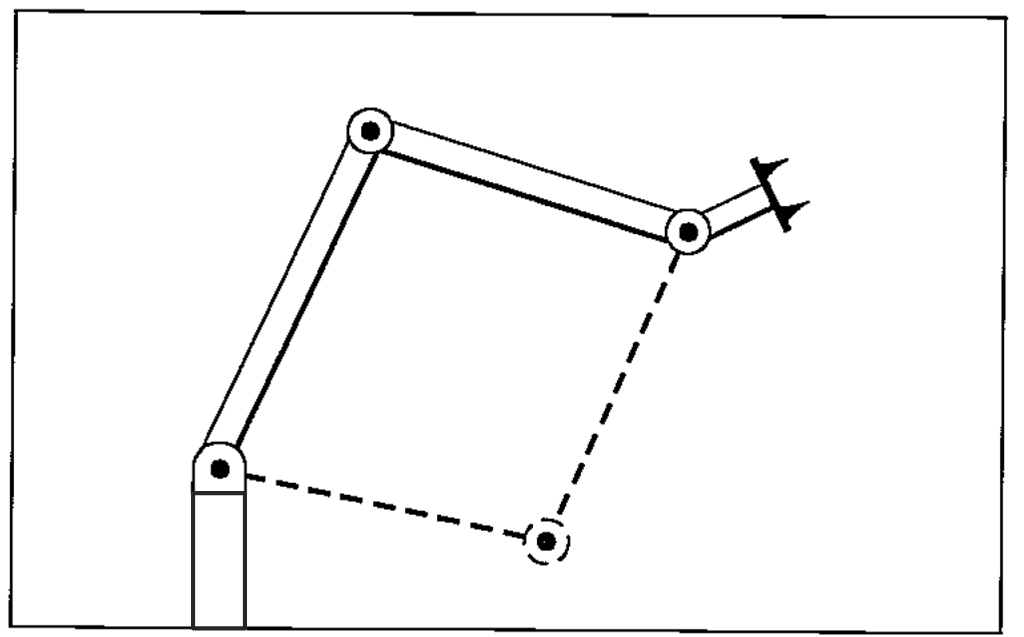
\includegraphics[
	width=1\linewidth,
	center,
	keepaspectratio,
	]{invKin/Multip_Sol}
	\caption{Three link manipulator with 2 solutions}
	\label{fig:multipSol3Link}
\end{figure}

This can be extended to the 6\ac{DOF} serial link manipulators.
As stated by YanWu et al. there are 8 groups of inverse solution for most \ac{EOAT}-positions within the manipulator's workspace \cite{invKinSolYanWu}. 

\begin{figure}[H]
	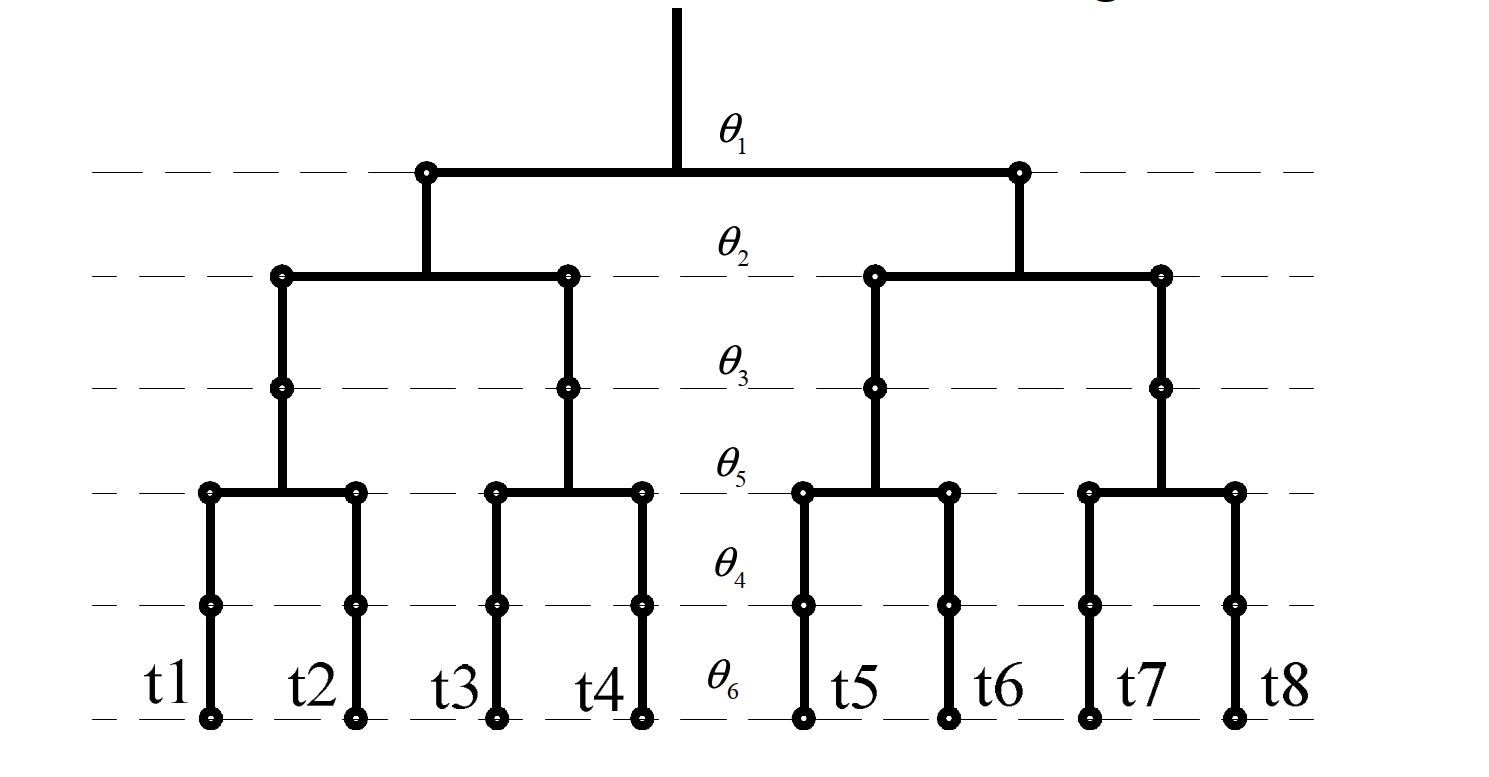
\includegraphics[
	width=1\linewidth,
	center,
	keepaspectratio,
	]{invKin/TreeOfInvserseSolution}
	\caption{Tree of inverse solutions (\cite{invKinSolYanWu}, fig.2)}
	\label{fig:invKinTree}
\end{figure}

\section{Inverse solution of 6 \ac{DOF} Robot}

As shown in chapter \ref{ForKinEq} the end effector position is defined by four vectors $ (n,o,a,p) $. With these known, the joint variables $(\theta_1, \theta_2, \theta_3, \theta_4, \theta_5, \theta_6)$ can be calculated.
This problem  is solved by the method of using the inverse transformation of unknown link pre-multiplication as presented by Yan Wu et al. \cite{invKinSolYanWu}. 

\paragraph{Forward kinematic equation}
For a 6\ac{DOF} Robot, the  forward kinematic matrix equation from equation \cref{eq:SummofTranfMatr,eq:matrixForm} can be reformulated into equation \ref{eq:ForwKinEquMatr}

\begin{equation}\label{eq:ForwKinEquMatr}
	^0_6T = \\
	\begin{bmatrix}
n_x & o_x & a_x & p_x \\
n_y & o_y & a_y & p_y \\
n_z & o_z & a_z & p_z \\
0 & 0 & 0 & 1 \\
\end{bmatrix}
=
\phantom{}^0_1T(\theta_1)\phantom{}^1_2T(\theta_2)\phantom{}^2_3T(\theta_3)\phantom{}^3_4T(\theta_4)\phantom{}^4_5T(\theta_5)\phantom{}^5_6T(\theta_6)\\
\end{equation}

\section{The inverse Solution} \label{InverseSol}
With $ (n,o,a,p) $ known, the angle values of the joint variables can be determined by separation of the joint variables. 
In a first step \ac{eq} \ref{eq:ForwKinEquMatr} is reformed into \ac{eq} \ref{eq:ForwKinEquMatr_reformed}.
\begin{equation}\label{eq:ForwKinEquMatr_reformed}
	\phantom{}^2T_3\phantom{}^3T_4\phantom{}^4T_5 = \phantom{}^0T_6(\phantom{}^0T_1)^{-1}(\phantom{}^1T_2)^{-1}(\phantom{}^5T_6)^{-1}
\end{equation}
This gives 2 matrices, formed by the terms found in eq \ref{eq:TransformMatrices_0-6}. These matrices are the terms found in \ac{eq}\ref{eq:ForwKinEquMatr_reformed}.
With the help of MATLAB and the symbolic toolbox, the inverses and the overall product of each side can be calculated. %should be done for actual confirmation. Test it!

	

\begin{multline}\label{eq:prelinkmultip_right}
	\phantom{}^2T_3\phantom{}^3T_4\phantom{}^4T_5 =\\
	\NiceMatrixOptions{
		code-for-first-row= \color{red},
		code-for-first-col= \color{green},
%		code-for-last-row= \color{blue},
%		code-for-last-col= \color{magenta}
	}
	\begin{pNiceArray}{C:C:C:C}[first-row,first-col] %[first-row,last-row,first-col,last-col]
%	\begin{bmatrix}
& 1 & 2 & 3 & 4 \\
1 & 	\parbox{0.2\linewidth}{$ c_3 c_4 c_5 - s_3 s_5 $} & \parbox{0.2\linewidth}{$  -c_3 c_4 s_5 - s_3 c_5 $} & \parbox{0.2\linewidth}{$  c_3 s_4 $} & \parbox{0.2\linewidth}{$  c_3 a_3 - s_3 d_4 + a_2 $} \\ \hdottedline
2 & 	\parbox{0.2\linewidth}{$ s_3 c_4 c_5 + c_3 s_5 $} & \parbox{0.2\linewidth}{$  -s_3 c_4 s_5 + c_3 c_5 $} & \parbox{0.2\linewidth}{$  s_3 s_4 $} & \parbox{0.2\linewidth}{$ s_3 a_3 + c_3 d_4 $} \\ \hdottedline
3 & 	\parbox{0.2\linewidth}{$ -s_4 c_5 $} & \parbox{0.2\linewidth}{$  s_4 s_5 $} & \parbox{0.2\linewidth}{$  c_4 $} & \parbox{0.2\linewidth}{$  0 $} \\ \hdottedline
4 & 	\parbox{0.2\linewidth}{$ 0 $} & \parbox{0.2\linewidth}{$  0 $} & \parbox{0.2\linewidth}{$  0 $} & \parbox{0.2\linewidth}{$  1 $} \\
%	\end{bmatrix}
\end{pNiceArray}
\end{multline}
%& A & B & C & D\\
%1 & 	c_3 c_4 c_5 - s_3 s_5 & -c_3 c_4 s_5 - s_3 c_5 & c_3 s_4 & c_3 a_3 - s_3 d_4 + a_2 \\
%2 & 	s_3 c_4 c_5 + c_3 s_5 & -s_3 c_4 s_5 + c_3 c_5 & s_3 s_4 & s_3 a_3 + c_3 d_4 \\
%3 & 	-s_4 c_5 & s_4 s_5 & c_4 & 0 \\
%4 & 	0 & 0 & 0 & 1 \\
\medskip
\begin{multline}\label{eq:prelinkmultip_left}
	\phantom{}^0T_6(\phantom{}^0T_1)^{-1}(\phantom{}^1T_2)^{-1}(\phantom{}^5T_6)^{-1} =\\
	\begin{pNiceArray}{C:C:C:C}
%\begin{bmatrix}
	\parbox{0.25\linewidth}{$ (c_2 c_1 n_x + c_2 s_1 n_y - s_2 n_z)c_6 - (c_2 c_1 o_x + c_2 s_1 o_y -s_2 o_z) s_6 $} & 
	\parbox{0.2\linewidth}{$ c_2 c_1 a_x + c_2 s_1 a_y - s_2 a_z $} &
	\parbox{0.25\linewidth}{$ -(c_2 c_1 n_x + c_2 s_1 n_y - s_2 n_z) s_6 - (c_2 c_1 o_x + c_2 s_1 o_y - s_2 o_z) c_6 $} &
	\parbox{0.25\linewidth}{$ -(c_2 c_1 a_x + c_2 s_1 a_y - s_2 a_z ) d_6 + c_2 c_1 p_x + c_2 s_1 p_y - s_2 p_z -c_2 a_1 $} 
	\\\hdottedline
	\parbox{0.25\linewidth}{$ -(s_2 c_1 n_x - s_2 s_1 n_y - c_2 n_z) c_6 - (-s_2 c_1 o_x - s_2 s_1 o_y - c_2 o_z) s_6 $} &
	\parbox{0.2\linewidth}{$ -s_2 c_1 a_x - s_2 s_1 a_y -c_2 a_z $} & 
	\parbox{0.25\linewidth}{$ -(-s_2 c_1 n_x -s_2 s_1 n_y -c_2 n_z) s_6 - (- s_2 c_1 o_x - s_2 s_1 o_y - c_2 o_z)c_6 $} &
	\parbox{0.25\linewidth}{$ -(-s_2 c_1 a_x - s_2 s_1 a_y - c_2 a_z)d_6 - s_2 c_1 p_x - s_2 s_1 p_y - c_2 p_z +s_2 a_1 $}
	\\ \hdottedline
	\parbox{0.25\linewidth}{$ ( -s_1 n_x + c_1 n_y) c_6 - (-s_1 o_x + c_1 o_y) s_6 $} &
	\parbox{0.2\linewidth}{$ - s_1 a_1 + c_1 a_2 $} &
	\parbox{0.25\linewidth}{$ -(-s_1 n_x + c_1 n_y ) s_6 -(-s_1 o_x + c_1 o_y ) c_6 $} &
	\parbox{0.25\linewidth}{$ -(-s_1 a_x + c_1 a_y) d_6 - s_1 p_x + c_1 p_y $} 
	\\ \hdottedline
	\parbox{0.25\linewidth}{$ 0 $} &
	\parbox{0.2\linewidth}{$ 0 $} &
	\parbox{0.25\linewidth}{$ 0 $} &
	\parbox{0.25\linewidth}{$ 1 $}
	\\
%\end{bmatrix}
	\end{pNiceArray}
\end{multline}
In equations \cref{eq:prelinkmultip_right,eq:prelinkmultip_left} $sin(\theta_i) $ and $ \cos(\theta_i) $ have been replaced by $s_i$ and $c_i$ to allow for appropriate presentation of the matrix. This abbreviation will be used for following steps as well. \\
\medskip
%\s*(TODO|Check when to use which bracket type []() for matrices, bmatrix pmatrix)


As shown by eq. \ref{eq:ForwKinEquMatr_reformed}, the elements of matrices \cref{eq:prelinkmultip_right,eq:prelinkmultip_left} are corresponding equal. This allows to find analytic expressions for all $\theta_i$. As stated in section \ref{MultipSol}, there are two solutions for each $\theta_i$.
\medskip


\paragraph{$\theta_1$:}

By taking the elements (\textcolor{green}{3},\textcolor{red}{4}) of equations \cref{eq:prelinkmultip_right,eq:prelinkmultip_left} as corresponding equal, equation \ref{eq:equal_3-4} is formed.
\begin{equation}\label{eq:equal_3-4}
	-(-s_1a_x + c_1 a_y )d_6 - s_1 p_x +c_1 p_y = 0
\end{equation}
Reforming equation \ref{eq:equal_3-4} gives a solution for $\theta_1$ as seen in equation \ref{eq:sol_theta_1}.
\begin{multline}\label{eq:sol_theta_1}
	\theta_{1_1} = \atantwo ( p_y - a_y d_6 , p_x - a_x d_6) 
	\phantom{......}
	\theta_{1_2} = \atantwo (-p_y + a_y d_6 ,-p_x + a_x d_6) 
\end{multline}
\medskip

\paragraph{$\theta_2$:}

Taking elements (\textcolor{green}{1},\textcolor{red}{4}) and (\textcolor{green}{2},\textcolor{red}{4}) of equations \cref{eq:prelinkmultip_right,eq:prelinkmultip_left} as corresponding equal, equations \ref{eq:equal_1-4} and \ref{eq:equal_2-4} are formed.
\begin{equation}\label{eq:equal_1-4}
	a_3 c_3 - d_4 s_3 + a_2 = - (c_2 c_1 a_x + c_2 s_1 a_y -s_2 a_z)d_6 + c_2 c_1 p_x + c_2 s_1 p_y -s_2 p_z -c_2 a_1
\end{equation}
\begin{equation}\label{eq:equal_2-4}
	a_3 s_3 +d_4 c_3 = - (- s_2 c_1 a_x - s_2 s_1 a_y - c_2 a_z)d_6 s_2 c_1 p_x s_2 s_1 p_y  -c_2 p_z +s_2 a_1
\end{equation}
For simplification of the terms in equations \cref{eq:equal_1-4,eq:equal_2-4}, middle variables are chosen:
\begin{equation}
	u=c_1 (p_x d_6 a_x ) + s_1 (p_y -a_y d_6)-a_1 \phantom[...]
	v= p_z - a_z d_6
\end{equation}

With these middle variables equations \cref{eq:equal_1-4,eq:equal_2-4} can be rewritten as seen in \cref{eq:equal_1-4_midVar,eq:equal_2-4_midVar}.
\begin{equation}\label{eq:equal_1-4_midVar}
	a_3 c_3 - d_4 s_3 = c_2 u -s_2 v -a_2 
\end{equation}
\begin{equation}\label{eq:equal_2-4_midVar}
	a_3 s_3 + d_4 c_3 = - s_ u - c_2 v
\end{equation}
To eliminate $s_3$ and $c_3$ equations \cref{eq:equal_1-4_midVar,eq:equal_2-4_midVar} are squared and then added to form \ref{eq:1-4+2_4}.
\begin{equation}\label{eq:1-4+2_4}
	a_3^2 +d_4^2 = u^2 +v^2 - 2a_2 c_2 u + 2a_2 s_2 v +a_2^2
\end{equation}
\begin{equation}\label{eq:1-4+2_4_reformed}
	\frac{a_3^2 + d_4^2 - u^2 - v^2 -a_2^2}{-2a_2}= c_2 u -s_2 v
\end{equation}
This equation can be further simplified by taking another middle variable:
\begin{equation*}
	m = \frac{a_3^2 +d_4^2 - u^1 -v^2 - a_2^2}{-2a_2}
\end{equation*}
Reforming equation \ref{eq:1-4+2_4_reformed} and inserting the middle variable reveals a solution for $\theta_2$ as seen in eq\ref{eq:sol_theta_2}.
\begin{equation}\label{eq:sol_theta_2}
	\theta_{2_{1/2}} = \atantwo (-v , u)\pm \atantwo(\sqrt{v^2 +u^2 - m^2 } , m)
\end{equation}



\paragraph{$\theta_3$:}

To recive $\theta_3$ it helps to take equations \cref{eq:equal_1-4,eq:equal_2-4}. Equation \ref{eq:equal_1-4} needs to be reformed into \ref{eq:eqal_1-4_reformed}
\begin{equation} \label{eq:eqal_1-4_reformed}
	a_c c_3 d_4 s_3 + a_2 = c_2 u -s_2 v
\end{equation}
Squaring of equations \cref{eq:eqal_1-4_reformed,eq:equal_2-4} and adding them eliminates $s_2$ and $c_2$ as seen in eq \ref{eq:1-4_reformed+2_4}
\begin{equation}\label{eq:1-4_reformed+2_4}
	a_2^2 + a_3^2 +d_4^2 + 2 a_2(a_3 c_3 -d_4 s_3) = u^2 + v^2
\end{equation}
\begin{equation}\label{eq:1-4_reformed+2_4_reformed}
	a_3 c_3 - d_4 s_3 = \frac{a_3^2 + d_4^2 - u^2 -v^2 +a_2^2}{2a_2}
\end{equation}

Again, this equation can be further simplified by taking another middle variable:
\begin{equation*}
	-\frac{a_3^2 + d_4^2 - u^2 -v^2 + a_2^2}{2a_2}
\end{equation*}

Reforming equation \ref{eq:1-4_reformed+2_4_reformed} and inserting the middle variable reveals a solution for $\theta_3$ as seen in eq\ref{eq:sol_theta_3}.
\begin{equation}\label{eq:sol_theta_3}
	\theta_{3_{1/2}} = \atantwo(-d_4 , a_3) \pm A \tan (2 (\sqrt{d_4^2 +a_3^2 -h^2} , h))
\end{equation}


\paragraph{$\theta_5$:}
Taking elements (\textcolor{green}{2},\textcolor{red}{2}) and (\textcolor{green}{1},\textcolor{red}{2}) of equations \cref{eq:prelinkmultip_right,eq:prelinkmultip_left} as corresponding equal, equations \ref{eq:equal_2-2} and \ref{eq:equal_1-2} are formed.

\begin{equation}\label{eq:equal_2-2}
	-s_3 c_4 s_5 + c_3 c_5 = -c_1 s_2 a_x - s_1 s_2 a_y -c_2 a_z
\end{equation}
\begin{equation}\label{eq:equal_1-2}
	-c_3 c_4 s_5 - s_3 c_4 = c_1 c_2 a_x + s_1 c_2 a_y - s_2 a_z
\end{equation}

To combine equations \cref{eq:equal_2-2,eq:equal_1-2}, eq \ref{eq:equal_2-2} is multiplied with $c_3$ and eq \ref{eq:equal_1-2} is multiplied by $ s_2$. The resulting equations are then subtracted from each other giving eq \ref{eq:2-2+1-2}.
\begin{equation}\label{eq:2-2+1-2}
	c_5 = (-c_1 s_2 a_x - s_1 s_2 a_y -c_2 a_z) c_3 - (c_1 c_2 a_x +s_1 c_2 a_y - s_2 a_z) s_3
\end{equation}
Reforming equation \ref{eq:2-2+1-2} gives a solution for $\theta_5$ as seen in equation \ref{eq:sol_theta_5}.
\begin{equation}\label{eq:sol_theta_5}
	\theta_{5_{1/2}} = \pm \arccos [ ( -c_1 s_2 a_x - s_1 s_2 a_y - c_2 a_z) c_3 - (c_1 c_2 a_x + s_1 c_2 a_y - s_2 a_z) s_3]
\end{equation}

\paragraph{$\theta_4$:}

With $\theta_5$ and $\theta_{1-3}$ known, equation \ref{eq:equal_1-2} can be reformed into a solution for $\theta_4$ as seen in equation \ref{eq:sol_theta_4}
\begin{equation}\label{eq:sol_theta_4}
	\theta_{4_{1/}} = \pm \arccos [ \frac{ c_1 c_2 a_x + s_1 c_2 a_y - s_2 a_z + s_3 c_5}{-c_3 s_5}]
\end{equation}

\paragraph{$\theta_6$:}
By taking the elements (\textcolor{green}{3},\textcolor{red}{3}) of equations \cref{eq:prelinkmultip_right,eq:prelinkmultip_left} as corresponding equal, equation \ref{eq:equal_3-3} is formed.
\begin{equation} \label{eq:equal_3-3}
	s_6 (s_1 n_x - c_1 n_y) + c_6 (s_1 o_x - c_1 o_y ) = c_4
\end{equation}

With $\theta_4$ and $\theta_1$ known, equation \ref{eq:equal_3-3} can be reformed into a solution for $\theta_6$ as seen in equation \ref{eq:sol_theta_6}.
\begin{equation}\label{eq:sol_theta_6}
	\theta_{6_{1/2}} = \atantwo(s_1 n_x -c_1 n_y , s_1 o_x -c_1 o_y) \pm \atantwo(\sqrt{(s_1 n_x - c_1 n_y)^2 + (s_1 o_x - c_1 o_y )^2 - c_4^2} , c_4)
\end{equation}

With equations \cref{eq:sol_theta_1,eq:sol_theta_2,eq:sol_theta_3,eq:sol_theta_4,eq:sol_theta_5,eq:sol_theta_6} the values for $(\theta_1, \theta_2, \theta_3, \theta_4, \theta_5, \theta_6)$ can be calculated for all reachable end effector positions.

The $\atantwo(x,y)$-function used in this solution which returns an angle between the positive x axis and a line pointing to $(x,y) \neq (0,0)$. The function takes two arguments and returns a single value $\theta$ between $-\pi$ and $\pi$ equivalent to the phase angle of complex numbers. While $\arctan$ can only solve in quadrant 1 and 4, $\arctantwo$ allows for calculation in all four quadrants because it differentiates between pos/neg $x$  and  $y$ direction independently. It is mostly a question of implementation and solving method, so this new notation arose with programming languages.


\section{Optimization of inverse kinematics solution}

As stated in section \ref{MultipSol}, there exist eight sets of inverse solutions in the dextrous workspace (see \ref{ExistSol}).
The optimal solution can be found through an optimization function. 
This optimization function needs to find the set of solution that can reach the desired position fastest from the current position.\\
\\
\paragraph{cost function}
Equation \ref{eq:costFuncinvOptim} is the cost function to be minimized.
\begin{itemize}
	\item[$\theta_i (k+1)$:] target angle
	\item[$\theta_i(k)$:] departing angle
	\item[$k_i$] power value
\end{itemize}

\begin{equation}\label{eq:costFuncinvOptim}
	err =  \min\sum_{i=1}^{6} k_i [\theta_i (k+1) - \theta_i(k)] 
\end{equation}

As can be seen, this cost function minimizes the sum of angles over all axes for the movement of the end effector from position $[n_i,o_i,a_i,p_i ]$ to $[n_{i+1}, o_{i+1}, a_{i+1}, p_{i+1}]$ by using the inverse solution presented in chapter \ref{InverseSol}.

\paragraph{limitations of cost function}
This cost function not necessarily gives the fastest path, as it does not account for the actual movement speed of the different axes. 
A possible solution for this would require multiplying with a cost factor between 0 and 1 for each joint ( 1 for the slowest joint) with the respective angle error to account for the difference in angular velocity.



\paragraph{description of implementation}

An implementation of this function receives the current position either in joint angles or Cartesian coordinates of the end-effector which could be given in form of a rotation matrix as seen in eq\ref{eq:matrixForm} or in form of euclidean space and euler angle coordinates. $[x,y,z, \alpha, \beta, \gamma]$ which could be transformed by the inverse of equation \ref{eq:rotMatrix_composition} into a rotation matrix.

This algorithm would then start the calculation to get all possible paths in the tree of inverse solutions (see figure \ref{fig:invKinTree}) for position ${i+1}$.

\paragraph{algorithm for minimal computational effort}

To minimize the computational effort, following algorithm is proposed by Yan Wu et al. \cite{invKinSolYanWu}:

\begin{enumerate}
	\item The calculation starts with $\theta_1$ by finding the two solutions for equation \ref{eq:sol_theta_1}.
	\item When calculating $\theta_2$:
	\begin{enumerate}
		\item  The term $ v^2 + u^2 - m^2 $ should be $ > 0$, otherwise the program can terminate the calculation of the subsequent steps of this group, return $err = inf $ or $NaN $ , and provide a varible like $P=1$ to determine the cause for the abortion of subsequent steps.
		\item If there is a solution for $\theta_2$ it needs to be tested for extraneous roots. An extraneous root is  introduced into an equation in the process of solving another equation, but is not a solution of the equation to be solved \cite{extraneousroot}. This test is done simply by substituting the solution for $\theta_2$ into the original equation \ref{eq:1-4+2_4}. If an extraneous root is found, the program can terminate and return $err = inf$ or $ NaN$  and $P=2$ for cause of abortion. 
	\end{enumerate}
	\item If the calculation has been continued, $\theta_3$ can be determined. Again a test for extraneous roots is necessary.
	\item When calculating $\theta_5$, test for extraneous roots.
	\item When calculating $\theta_4$, test for extraneous roots.
	\item calculate $\theta_6$
	\item determine error as seen in eq \ref{eq:costFuncinvOptim} for all possible paths
	\item find $\min ( err(t_1^8))$ 
\end{enumerate}

The resulting set of angle values is the result of the algorithm. It is the unique inverse solution, determined easiest to reach with the given cost function in eq \ref{eq:costFuncinvOptim}. 





%https://robotics.stackexchange.com/questions/10322/is-it-possible-to-get-all-possible-solutions-of-verse-kinematics-of-a-6-dof-ar
%In general, if the wrist is spherical (i.e., all three axes intersect), you can enumerate all of the various closed-form solutions through a method known as wrist partitioning. This method uses the three arm joints to solve for the position of the wrist center. It then uses the wrist joints to determine the joint angles which orient the end effector properly. Multiple solutions are possible from "wrist up" and "wrist down" options, "elbow up" and "elbow down" options (for an articulated arm), and "over the shoulder" options also. For other robot geometries the options would differ.

%If the wrist is not spherical, it becomes quite challenging to find a closed-form inverse solution. But you still have the various geometric options for inverse kinematics solutions.
%
%One way to make sure you are identifying all of the solutions is to recall the fundamentals of trigonometry. Recall that sin(θ)=−sin(−θ)
%and cos(θ)=cos(−θ). So when you are solving for θ you have to consider the other angles which produce the same result using these and other trigonometric identities. 
	\chapter{\ac{DH}-Convention} \label{sec:DH-convention}

The \ac{DH}-Convention is a commonly used and simplifies the forward and backward transformation. It was named after Jaques Denavit and Richard Hartenberg who developed a general theory to describe a serial link mechanism. \cite{DenavitHartenbergLesson}\\
It consists of following parts:

\begin{itemize}[leftmargin=3cm]
	\item \ac{DH}-Convention for establishing the coordinate systems
	\item \ac{DH}-Transformation for generation of the coordinate systems
	\item \ac{DH}-Parameters as a result form the transformations
\end{itemize}

Determining the coordinate systems is done according to set rules. Nevertheless, the choices of coordinate frames are also not unique, so different people will derive different, but correct frame assignments. This freedom of choice should be used to bring as many \ac{DH}-Parameters as possible to zero. This simplifies subsequent equations and calculations. \cite{DenavitHartenbergKonventionen}

Each joint of the robot is described by four parameters.

This leads to a kinematic chain with each frame determined by the previous one \cite{DenavitHartenbergKonventionen}.\\
\\

Link0 - Link1 - Link2 - Link3 - Link4 - Link5 - Link6\\
\\

Each \ac{DH}-transformation consists of four elementary transformations\cite{DenavitHartenbergKonventionen}:

\begin{enumerate}[label=\emph{\arabic*)}]
	\item rotation around the $x_i$-axis with the amount of $\alpha_i$
	\item translation along $x_i$-axis with the amount of  $a_i$
	\item translation along $z_i$-axis with the amount of  $d_i$
	\item rotation around $z_i$-axis with the amount of  $\theta_i$
\end{enumerate}

This shows that the \ac{DH} robotic convention is a minimal line representation, as with four parameters, all possible lines in the Euclidean Space can be represented (\cite{AutRobVeh}, page 210).

Following from this, two pairs of parameters determine the joints and links \cite{ConstantinForwardKA}:
\begin{itemize}[wide=\parindent] 
	\item[Links:] represented by link length ($a$) and link twist ($\alpha$)
	%, defined as the relative location of the two attached joint axes.
	\item[Joints:] represented by link offset ($d$)
	% which is the distance from one link to the next 
	and joint angle ($\theta$) 
	%which is the rotation of one link with respect to the next around the joint axis.
\end{itemize}
\phantom{}\\

	
%	\input{ThesisWork/}
	
	
	\chapter{Robot configurations} \label{sec:RobConf}

As mentioned before, a 6 \ac{DOF} manipulator can reach the same position in multiple configurations.
The different configurations in the solutions can be seen in the example of the FANUC robot arms (see figure \ref{fig:RobotConfigs})
\medskip
%\begin{itemize}
%	\item Flip vs. No-Flip
%	\item Up vs. Down
%	\item Front vs. Back
%\end{itemize} \cite{OneRobFanucConfigurations}

\begin{figure}[H]
	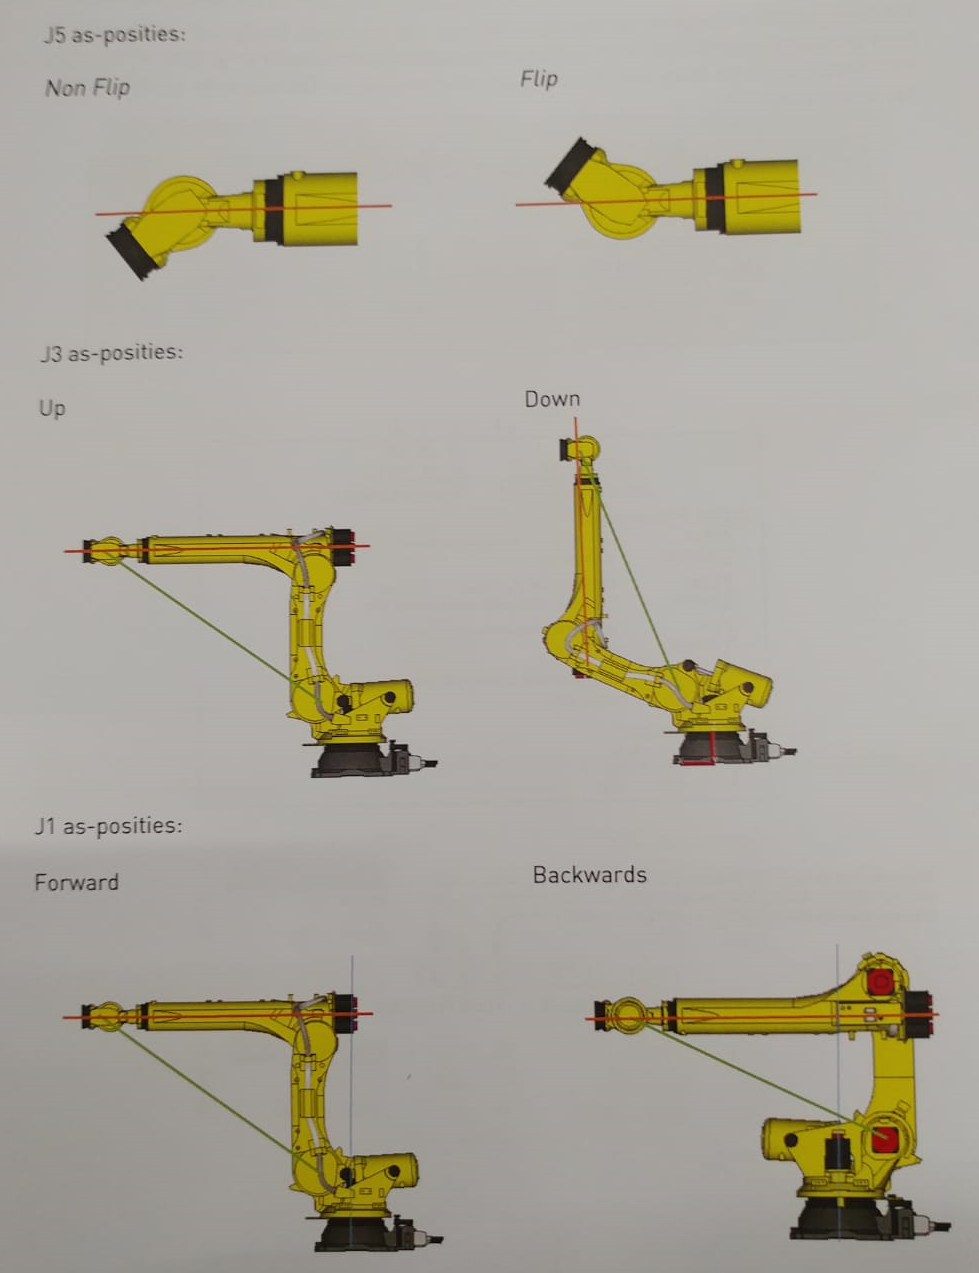
\includegraphics[
	width=0.6\linewidth,
	center,
	keepaspectratio,
	]{FanuRobotConfigurations_cr}
	\caption{6 axis robot configurations on the example of a FANUC Robot \cite{QingFanucAcademy}}
	\label{fig:RobotConfigs}
\end{figure}
\phantom{}\\
There exist $2^3=8$ solutions for the robot arm.

\phantom{}\\


	

	\renewcommand{\bibname}{References}
	\printbibliography
	\newpage
	
	
	\begin{appendices}
		\chapter{Appendix 1}
		\chapter{Appendix 2}
		%\chapter{Choice of IP address space}

%\url{https://en.wikipedia.org/wiki/Private_network}
 
It is in the class B of private IPv4 address space. Usually for home networks class c networks $ (192.168.0.0 – 192.168.255.255) $ are used. These allow to address$  256 $ adresses per subnet. without the gateway$  (.0) $ the broadcast address $ (.255) $ and an address for the router, we're left with 253 addresses. 
For the beginning, it might be an address space that is big enough, but if we include a lot of sensors, and other things, a space of 253 addresses might get small. 
 
Also this address space is usually used with a subnet mask of 255.255.0.0 which allows a mapping of  255 main addresses (172.x.0.x - 172.x.255.x) with 255 subpoints (172.x.x.0 - 172.x.x.255). Like this, each domain can get their own subnet (172.16.x.x-172.31.x.x), each device can get a main address space and then the different ports on the machines can be given numbers.
 
Also the  B block is not that commonly used, so this works also as a first line of defence against attachs from outside. Port knocking e.g. becomes harder, as the address space is way bigger.
		\chapter{Robot Quick start guide}
A big part of this was derived from \cite{MatlabControl}.

\section{Parts of the robot}
A quick overview over the visible parts.

\subsubsection{FANUC R-2000iC/210F 6 axis robotic arm}
The robot has 6 movable joints with a possible payload attached to the end. Its features include a wide reach (2655 mm), sturdy but flexible arm design, a spring loaded counterbalance, relatively high payload capacity (210Kg) and fast moving axes. The joints also have hashes to indicate the zero positions which help with the calibration of the robot. 

\subsection{R30iA Robot Controller }
The Robot is controlled using an original equipment manufacturer controller called the FANUC R30iA controller. Its features include faster sustained speed and superior position accuracies. It also has the I/O ports that are used to connect grippers and other payloads. (It also houses the camera circuits which are required to access the data from the SONY camera provided with the robot. - Delta only)  The controller is also provided with a data card slot in which the special SD cards manufactured can be inserted and used as external memory. On the outside of the controller (side of iPendant at Delta) a USB port can be found. With these, programs, firmware files and other files can easily be transferred. Additionally, there is extended connectivity via its Ethernet port e.g. for FTP available.

\subsection{iPendant}
The teaching pendant is the primary user interface to the robot. It is used to move the joints of the robot manually, to program specific trajectories, to control the gripper, and various other actions. It also is an interface that can be used for input and output of the robot controller parameters. The user can access the system variables and position variables. (It is provided with a USB port that can be used to connect to a USB drive for external storage. - Delta only) It can also be used to setup an FTP server and client in order to communicate with the PC. 

\subsubsection{Gripper}
The robot as handed over does not have an active gripper system. It has been tested though with a pneumatic gripper controlled via the DO ports and pneumatic valves. A 2-way pneumatic valve, some piping and a pressure regulator are still available. (Delta Equipment varies here a lot).


\section{iPendant Navigation Manual:}
The teaching pendant is the primary user interface to the robot. This section deals with the important 
buttons on the TP. 


\begin{figure}[H]
	\centering
	\includegraphics
	[width=0.8\linewidth
	]{images/iPendant_Numbered}
	\caption[Important buttons]{Most important iPendant buttons numbered: This image from another iPendant than the ones available was chosen because of its labelling of buttons. Some buttons of the available iPendants are not labelled, so this picture can be used as a reference. Source: \cite{MatlabControl}}
	\label{fig:ipendantnumbered}
\end{figure}


\subsection{Emergency stop: }

Makes the robot stop immediately by applying brakes. Use it only when necessary as the brakes wear down. There is also an E-stop on the controller.
Press down on the button to activate it.
Twist it to the right to release.
If a slow and gradual halt is required, press HOLD on the iPendant.
TP on/off
Below the E-stop button. It should be ON to access any function in the Teach Pendant (Set-ups, calibration, programs etc) and OFF when running in AUTO mode.
Deadman switch
The 2 yellow bars behind the iPendant. 3 modes are available: Fully released, halfway pressed, fully pressed. Only the middle mode activates control.







		%\newpage
\chapter{IOT Projects:}

The \ac{SPC} is a research lab, that is in constant development to show the latest innovations and bring them to use in industrial applications.
In the context of the master-thesis "Using FANUC R-2000iC/210F (6-axis robot) for improved efficiency in FRC parts formation" the topic of digital twinning and with that \ac{IOT} has become a major research point. 
In order to bring the \ac{FRC} production line to its full potential, several new projects could be defined. 
These projects improve comfort, energy-efficiency, ease of use and safety of the lab.
Each of these projects is designed to provide a flexible workload for 1-3 students with varying results depending on the students experience level and semester. In case 3 students sign up for a project, the diligence work is expected to be fulfilled. Each student is expected to pick their own range of tasks that they fulfil.
Following project ideas are proposed:\\
\bigskip
%
\section*{Room Temperature Control System}

	\begin{figure}[H]
	\centering
	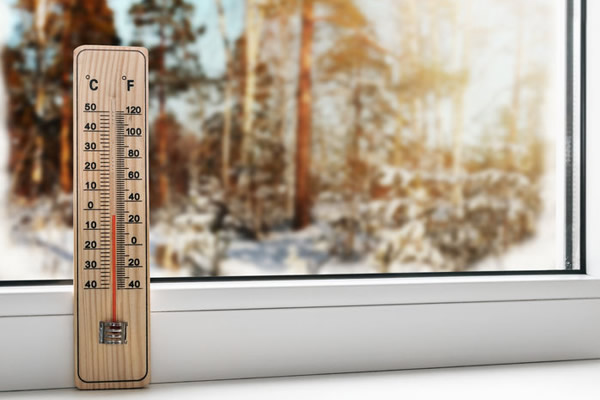
\includegraphics[
	width=0.5\linewidth,
	height=\paperheight,
	keepaspectratio,
	]{RoomTemp}
	\caption{Heating when noone needs it is waste! \cite{RoomTemp}}
	\label{fig: RoomTemp}
\end{figure}


The Lab of the \ac{SPC} has an old heating system controlled with electromechanical thermostats. 
Originally this system was designed to work with steam delivered by the \ac{IPKW}. 
Later this System was retrofitted with two gas heaters that have no feedback about the actual heating demand. This needs to be improved for comfort and energy-efficiency.\\
\\
Your assignment will be to replace the old and manual control with an open-source home automation system. That means choosing sensors, actuators, electronic components and clients as well as the type of home automation servers. 
A possible approach would be using thermocouples as sensors, transistors to switch the inputs of the heating system, using an ESP8266 for sensing and controlling with \ac{FHEM} as the underlying home automation server running on a raspberry pi.\\
diligence work: also include other room thermostats in the offices as well as lights\\
\\
Why are you the right one for this project? (Not all is required, but some should resonate with you)
\begin{itemize}
\item You are interested in automation systems
\item You like improving existing systems with electronics
\item You have experience with Arduino/ESP8266
\item You are not afraid to learn a new programming language to do some basic tasks
\item You like Linux
\item You like it warm and cozy in the morning :)
\end{itemize}
\bigskip
%
\section*{NFC based Machine Access}

	\begin{figure}[H]
	\centering
	
\includegraphics[
	width=0.5\linewidth,
	height=\paperheight,
	keepaspectratio,
	]{NFC}
	\caption{\ac{NFC} \cite{NFC}}
	\label{fig: NFC}
\end{figure}


The Lab of the \ac{SPC} has several heavy machines that move at high velocities, apply high pressures or create high temperatures. Because of these and other risks, a zoned safety system would make the lab a lot safer, as people would then stay in their assigned working zones while leaving work at other places unaffected. Also machine access needs to be restricted to the assigned student, while still leaving a traceable, temporarily restricted access to other users if necessary.\\
\\
Your assignment will be creating a \ac{NFC} card based zone and machine access. You can base this on an existing framework, or do it yourself. You will set up several \ac{NFC} readers with microcontrollers. These microcontrollers need to send a signal to a server that compares the access parameters delivered from the \ac{NFC}-card with a database that you set up. In case of a match, a signal is sent back to the Arduino, that switches a relay to open the gate. Additionally the Arduino should listen to other inputs in case a product cycle needs to be finished or additional requirements need to be fulfilled. Also there should be a signal sent back, when someone checks out of a safety zone. Machine access should have a timeout. Make a nice frontend to manage access.\\
diligence work: Make the communication between server and client hard to hack\\
\\
Why are you the right one for this project? (Not all is required, but some should resonate with you)
\begin{itemize}
\item You are interested in safety/security systems
\item You like to integrate something new into an ongoing project
\item You have experience with programming
\item You like microcontrollers
\item You can make a \ac{GUI}
\item (For diligence work: You like crypto)
\end{itemize}
\bigskip
%
%\section{Visual tool management system}
%In the lab of the \ac{SPC} many students use different tools like hammer, screwdrivers, wrenches etc. These tools get used throughout the day but rarely find their way back to their designated places (I'm also guilty of this). After spending a long time in the lab, many tools loose their designated storage places. It would be handy to take a photo of a tool and receive information about where to store it. Additionally, through the database the catalogue of available tools could be searched. \\
%\\
%Your assignment will be the creation of a program that can take a photo of a tool, recognize it and give out a description of its storage place with a photo. You will create a computer vision tool, probably based on machine learning to recognize the wide palette of tools in the lab.\\
%diligence work: Make it an android app\\
%\\
%Why are you the right one for this project? (Not all is required, but some should resonate with you)
%\begin{itemize}
%\item You are interested in image recognition
%\item You like to come up with something new
%\item You have experience with programming, ideally in Python
%\item (Diligence work: You would like to make an app)
%\item You don't like hardware
%\item You hate looking for stuff ;-)
%\end{itemize}
%\bigskip
%%
	\end{appendices}
	
	
	
\end{document}

%Questions for Report writing:Ton.ammerlaan@han.nl
